% arara: xelatex
%% arara: xelatex


% https://koalatea.io/r-knn-regression/
% http://freerangestats.info/blog/2017/04/09/propensity-v-regression
% https://economics.stackexchange.com/questions/45335/what-is-the-difference-between-ate-and-att
% https://kosukeimai.github.io/MatchIt/articles/matching-methods.html


\documentclass[14pt,xcolor=dvipsnames,handout]{beamer}


% !TEX root = om_metrics_14.tex

%\usepackage{epsdice} % dice 1-6 for probability :)

% \usepackage[absolute,overlay]{textpos}

% \usefonttheme[onlymath]{serif}

\usefonttheme{professionalfonts}
% by default beamer changes math fonts for better visibility for projection
% this professionalfonst theme removes this behavior


\usepackage[orientation=portrait,size=custom,width=25.4,height=19.05]{beamerposter}




%25,4 см 19,05 см размеры слайда в powerpoint

\usetheme{metropolis}
\metroset{
  %progressbar=none,
  numbering=none,
  subsectionpage=progressbar,
  block=fill
}

%\usecolortheme{seahorse}

\usepackage{fontspec}
\usepackage{polyglossia}
\setmainlanguage{russian}


% \usepackage{fontawesome5} % removed [fixed]
\setmainfont[Ligatures=TeX]{Myriad Pro}
% \setsansfont{Myriad Pro}




% why do we need \newfontfamily:
% http://tex.stackexchange.com/questions/91507/
\newfontfamily{\cyrillicfonttt}{Myriad Pro}
\newfontfamily{\cyrillicfont}{Myriad Pro}
%\newfontfamily{\cyrillicfontbs}{Myriad Pro}
\newfontfamily{\cyrillicfontsf}{Myriad Pro}


% https://tex.stackexchange.com/questions/175860/why-does-unicode-math-break-the-kerning-of-accents-in-combination-with-amssymb
% "You shouldn't be using amssymb together with unicode-math"
\usepackage{amsmath}
\usepackage{amsthm} % amssymb 


% https://tex.stackexchange.com/questions/483722/
% \usepackage[MnSymbol]{mathspec}  % Includes amsmath.
% \usepackage{mathspec}  % Includes amsmath.
% \setmathsfont(Digits,Latin,Greek,Symbols)[Numbers={Lining,Proportional}]{Latin Modern Math}
% mathspec must be loaded earlier than amsmath



%\usepackage{bm}

% \usepackage{fdsymbol} % \nperp

% \usepackage{unicode-math} % \symbf
% \setmathfont{Latin Modern Math}



\usepackage{centernot}

\usepackage{graphicx}

\usepackage{wrapfig}
% \usepackage{animate} % animations :)
% \usepackage{tikz}
%\usetikzlibrary{shapes.geometric,patterns,positioning,matrix,calc,arrows,shapes,fit,decorations,decorations.pathmorphing}
% \usepackage{pifont}
\usepackage{comment}
\usepackage[font=small,labelfont=bf]{caption}
\captionsetup[figure]{labelformat=empty}
% \includecomment{techno}



%Расположение

\setbeamersize{text margin left=15 mm,text margin right=5mm} 
\setlength{\leftmargini}{38 pt}

%\usepackage{showframe}
%\usepackage{enumitem}
% \setlist{leftmargin=5.5mm}


%Цвета от дирекции

\definecolor{dirblack}{RGB}{58, 58, 58}
\definecolor{dirwhite}{RGB}{245, 245, 245}
\definecolor{dirred}{RGB}{149, 55, 53}
\definecolor{dirblue}{RGB}{0, 90, 171}
\definecolor{dirorange}{RGB}{235, 143, 76}
\definecolor{dirlightblue}{RGB}{75, 172, 198}
\definecolor{dirgreen}{RGB}{155, 187, 89}
\definecolor{dircomment}{RGB}{128, 100, 162}

\setbeamercolor{title separator}{bg=dirlightblue!50, fg=dirblue}

%Цвета блоков

% Голубой блок!
\setbeamercolor{block title}{bg=dirblue!30,fg=dirblack}
\setbeamercolor{block title example}{bg=dirlightblue!50,fg=dirblack}
\setbeamercolor{block body example}{bg=dirlightblue!20,fg=dirblack}

\AtBeginEnvironment{exampleblock}{\setbeamercolor{itemize item}{fg=dirblack}}
%\setbeamertemplate{blocks}[rounded][shadow]

% Набор команд для удобства верстки

% Набор команд для структуризации

%\newcommand{\quest}{\faQuestionCircleO}
%\faPencilSquareO \faPuzzlePiece \faQuestionCircleO  \faIcon*[regular]{file} {\textcolor{dirblue}
%\newcommand{\quest}{\textcolor{dirblue}{\boxed{\textbf{?}}}
%\newcommand{\task}{\faIcon{tasks}}
%\newcommand{\exmpl}{\faPuzzlePiece}
%\newcommand{\dfn}{\faIcon{pen-square}}
%\newcommand{\quest}{\textcolor{dirblue}{\faQuestionCircle[regular]}}
%\newcommand{\acc}[1]{\textcolor{dirred}{#1}}
%\newcommand{\accm}[1]{\textcolor{dirred}{#1}}
%\newcommand{\acct}[1]{\textcolor{dirblue}{#1}}
%\newcommand{\acctm}[1]{\textcolor{dirblue}{#1}}
%\newcommand{\accex}[1]{\textcolor{dirblack}{\bf #1}}
%\newcommand{\accexm}[1]{\textcolor{dirblack}{ \mathbf{#1}}}
%\newcommand{\acclp}[1]{\textcolor{dirorange}{\it #1}}
\newcommand{\todo}[1]{\textcolor{dircomment}{\bf #1}}
%\newcommand{\graylink}[1]{{\fontsize{11}{12}\selectfont \textcolor{gray}{#1}}}
%\newcommand{\figcaption}[1]{{\fontsize{18}{20}\selectfont #1}}


\newcommand{\videotitle}[1]{
    {\fontsize{33}{30}\selectfont \textcolor{dirblue}{\textbf{#1}} }

    %\todo{название видеофрагмента}
}

\newcommand{\lecturetitle}[1]{
  {\fontsize{33}{30}\selectfont \textcolor{dirblue}{\textbf{#1}} }

    %\todo{название лекции}
}





%\newcommand{\spcbig}{\vspace{-10 pt}}
%\newcommand{\spcsmall}{\vspace{-5 pt}}

%\usepackage{listings}
%\lstset{
%xleftmargin=0 pt,
%  basicstyle=\small, 
%  language=Python,
  %tabsize = 2,
%  backgroundcolor=\color{mc!20!white}
%}



%\newcommand{\mypart}[1]{\begin{frame}[standout]{\huge #1}\end{frame}}

\setbeamercolor{background canvas}{bg=}

% frame title setup
\setbeamercolor{frametitle}{bg=,fg=dirblue}
\setbeamertemplate{frametitle}[default][left]

\addtobeamertemplate{frametitle}{\hspace*{0.1 cm}}{\vspace*{0.25cm}}


%Шрифты
\setbeamerfont{frametitle}{family=\rmfamily,series=\bfseries,size={\fontsize{33}{30}}}
\setbeamerfont{framesubtitle}{family=\rmfamily,series=\bfseries,size={\fontsize{26}{20}}}


% удобнее знать номер слайда, чтобы вносить правки!  

\setbeamercolor{footline}{fg=dircomment}
\setbeamerfont{footline}{series=\bfseries, size={\fontsize{12}{14}}}
%\setbeamertemplate{footline}[page number]


\defbeamertemplate{footline}{custom footline}
{%
  \hspace*{\fill}%
  \usebeamercolor[fg]{page number in head/foot}%
  \usebeamerfont{page number in head/foot}%
  page: \insertpagenumber\,/\,\insertpresentationendpage%
  \hspace{20pt}%
  slide: \insertframenumber\,/\,\inserttotalframenumber%
  %\hspace*{\fill}
  \vskip2pt%
}
%\setbeamertemplate{footline}[custom footline]

\usepackage{physics}
\usepackage[makeroom]{cancel}



% tikz block

\usepackage{pgfplots}
\pgfplotsset{compat=newest}

\usepackage{tikz}
\usetikzlibrary{calc}
\usetikzlibrary{quotes,angles}
\usetikzlibrary{arrows}
\usetikzlibrary{arrows.meta}
\usetikzlibrary{positioning,intersections,decorations.markings}
\usetikzlibrary{patterns}

\usepackage{tkz-euclide} 
%\tikzset{>=latex}

\tikzset{cross/.style={cross out, draw=black, minimum size=2*(#1-\pgflinewidth), inner sep=0pt, outer sep=0pt},
%default radius will be 1pt. 
cross/.default={5pt}}

\colorlet{veca}{red}
\colorlet{vecb}{blue}
\colorlet{vecc}{olive}


\newcommand{\grid}{\draw[color=gray,step=1.0,dotted] (-2.1,-2.1) grid (9.6,6.1)}

% end tikz block

\newcommand{\R}{\mathbb{R}}
\newcommand{\Rot}{\mathrm{R}}
\newcommand{\HH}{\mathrm{H}}
\newcommand{\Id}{\mathrm{I}}
\newcommand{\RR}{\mathbb{R}}
\newcommand{\ZZ}{\mathbb{Z}}
\newcommand{\la}{\lambda}
\let\P\relax
\newcommand{\P}{\mathbb{P}}
\newcommand{\E}{\mathbb{E}}

\newcommand{\cN}{\mathcal{N}}
\newcommand{\dN}{\mathcal{N}}

\newcommand{\qL}{q_{\text{left}}}
\newcommand{\qR}{q_{\text{right}}}



\newcommand{\ba}{\mathbf{a}}
\newcommand{\be}{\mathbf{e}}
\newcommand{\bb}{\mathbf{b}}
\newcommand{\bc}{\mathbf{c}}
\newcommand{\bd}{\mathbf{d}}
\newcommand{\bx}{\mathbf{x}}
\newcommand{\bff}{\mathbf{f}} % \bf is already def
\newcommand{\bv}{\mathbf{v}}
\newcommand{\bzero}{\mathbf{0}}



\DeclareMathOperator{\Var}{Var}
\DeclareMathOperator{\sVar}{sVar}
\DeclareMathOperator{\Cov}{Cov}
\DeclareMathOperator{\sCov}{sCov}
\DeclareMathOperator{\sCorr}{sCorr}
\DeclareMathOperator{\pCorr}{pCorr}
\DeclareMathOperator{\Corr}{Corr}
\DeclareMathOperator{\Med}{Med}
\let\L\relax
\DeclareMathOperator{\L}{L}


\DeclareMathOperator{\plim}{plim}
\DeclareMathOperator{\sign}{sign}


\newcommand{\graylink}[1]{{\fontsize{11}{12}\selectfont \textcolor{gray}{#1}}}
\newcommand{\figcaption}[1]{{\fontsize{18}{20}\selectfont #1}}





\begin{document}


\begin{frame} % название лекции


\lecturetitle{ARIMA processes}

\end{frame}


% !TEX root = ../om_ts_002.tex

\begin{frame} % название фрагмента

\videotitle{Stationary processes}

\end{frame}



\begin{frame}{Stationary processes: Plan}
  \begin{itemize}[<+->]
    \item Definition
    \item Random walk 
    \item Autocovariance function
    \item ACF, PACF
    
  \end{itemize}

\end{frame}

\begin{frame}
  \frametitle{Stationary processes}

   A stochastic process whose characteristics \alert{do not change over time}
  \pause

  \begin{block}{Weak or wide-sense stationarity}
    A process $(y_t)$  is said to be   \alert{weakly stationary}, if for each $t$ and $k$:
    \[
    \begin{cases}
      \E(y_t ) = \mu \\
      \Cov(y_t, y_{t+k}) = \gamma_k \\          
    \end{cases}
    \]
  \end{block}

  \pause
  \begin{block}{Strong or strict-sense stationarity}
    A process $(y_t)$  is said to be   \alert{ strictly stationary}, if for each  $k$ 
    joint  distribution of a r.v.  $(y_t, y_{t+1}, y_{t+2}, \ldots, y_{t+k})$ does not depend on  $t$
  \end{block}
\end{frame}




\begin{frame}
	\frametitle{Stationary process: example}
	
	\begin{block}{Independent observations}
		The quantities $(y_t)$ are independent and equally distributed
		with finite expectation $\mu_y$ and finite variance $\sigma^2_y$
	\end{block}
	
	\pause
	\[
	\mu_y = \E(y_t)
	\]
	\pause
	\[
	\gamma_0 = \Cov(y_t, y_t) = \Var(y_t) = \sigma^2_y
	\]
	\pause
	\[
	\gamma_k = \Cov(y_t, y_{t+k}) = 0, \text{ for } k \geq 1
	\]
\end{frame}



\begin{frame}
	\frametitle{Non-Stationary Process Example}
	
	\begin{block}{Random Walk}
		\[
		\begin{cases}
			y_0 = \mu \\
			y_t = y_{t-1} + u_t, \text{ for } t \geq 1 \\
		\end{cases},
		\]
		where $u_t$ is white noise
	\end{block}
	
	\pause
	
	\centering
	
	Explicitly: $y_t = \mu + u_1 + u_2 + \ldots + u_t$.
	\pause
	\[
	\mu_y = \E(y_t)
	\]
	\pause
	\[
	\gamma_0 = \Cov(y_t, y_t) = \Var(y_t) = \Var(\mu + u_1 + \ldots + u_t) = t\sigma^2_u
	\]
	\pause
	\[
	\gamma_k = \Cov(y_t, y_{t+k}) = \Cov(y_t, y_t + u_{t+1} + \ldots + u_{t+k}) = \Var(y_t)
	\]
\end{frame}

\begin{frame}
	\frametitle{Random Walk vs Random Sample}
	
	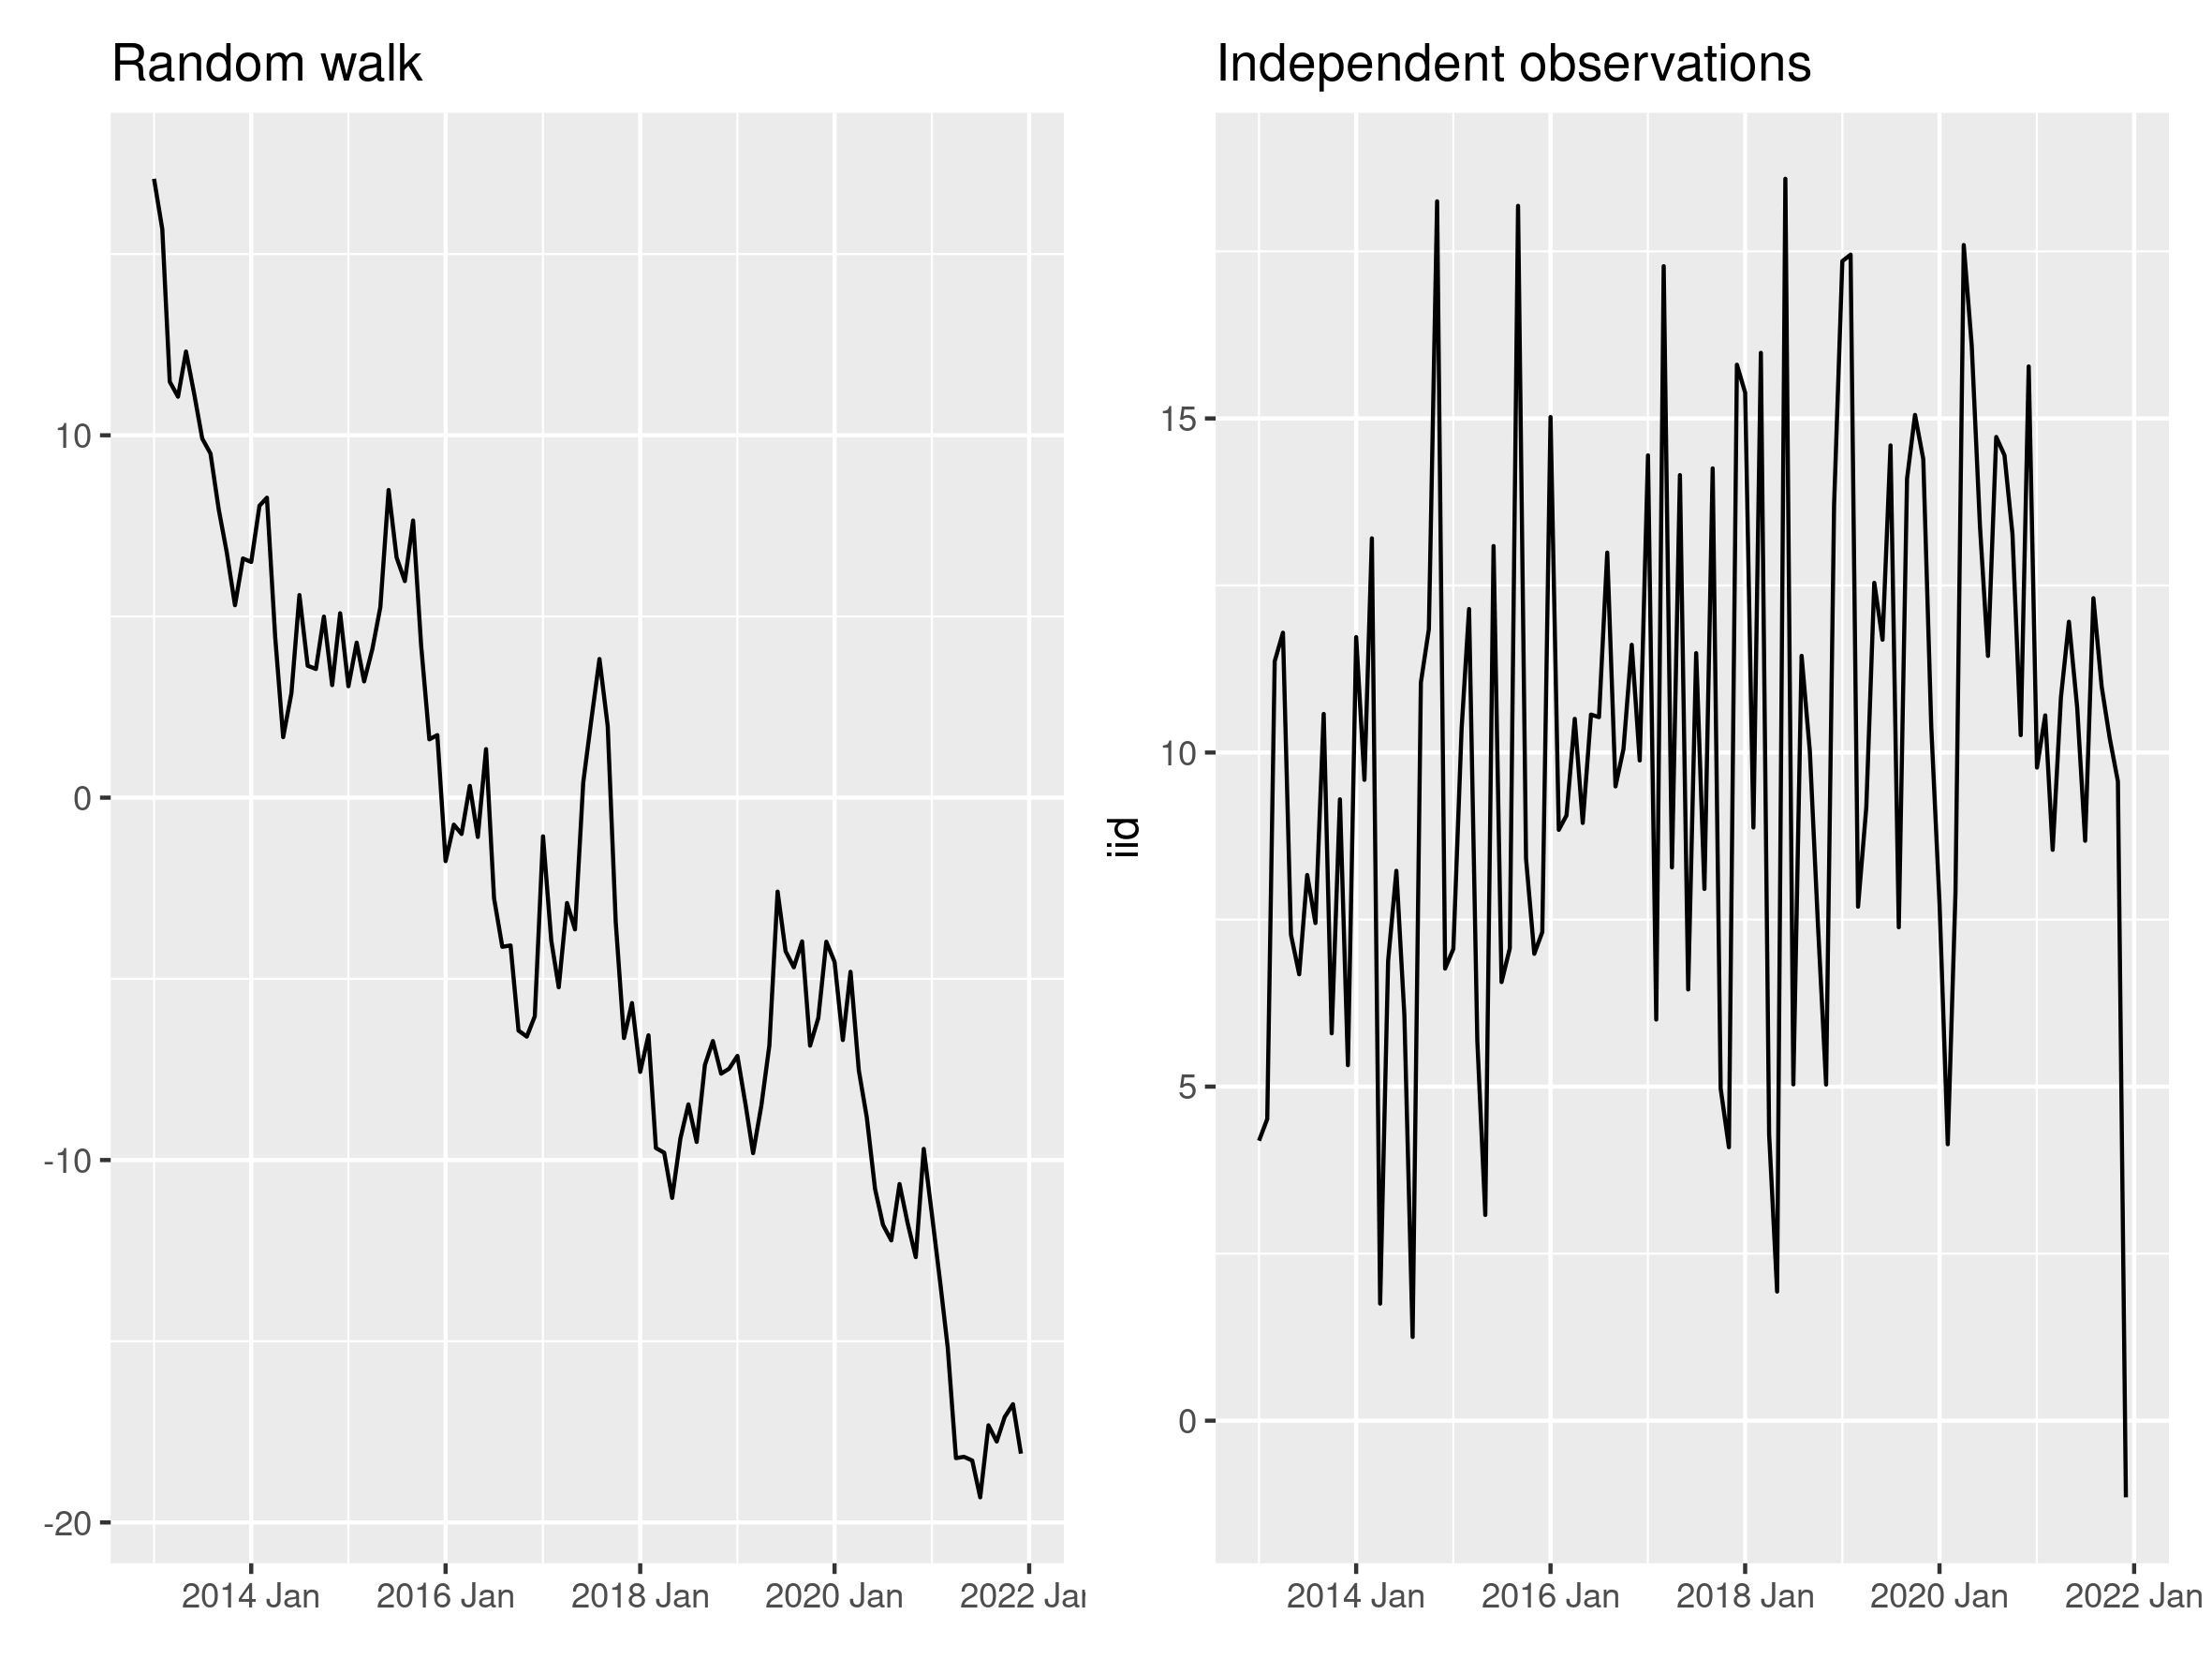
\includegraphics[width=\textwidth]{pictures/om_ts_04-028.png}
	
	
\end{frame}









\begin{frame}
	\frametitle{Autocovariance function}
	
	\begin{block}{Definition}
		For a stationary process $(y_t)$, the function $\gamma_k = \Cov(y_t, y_{t+k})$
		is called \alert{autocovariance}
	\end{block}
	
	\pause
	\begin{block}{Definition}
		For a stationary process $(y_t)$, the function $\rho_k = \Corr(y_t, y_{t+k})$
		is called \alert{autocorrelation}
	\end{block}
\end{frame}



\begin{frame}
\frametitle{ACF: autocorrelation function}
	
	\[
	\rho_k = \Corr(y_t, y_{y+j}) = \frac{\Cov(y_t, y_{y+j})}{\sqrt{\Var(y_t)\Var(y_{t+k})}} =  \pause
	\frac{\gamma_k}{\sqrt{\gamma_0 \gamma_0 }} = \frac{\gamma_k}{\gamma_0}
	\]  
	
\end{frame}




\begin{frame}
	\frametitle{Partial Correlation}
	
	\begin{block}{Definition}
		
		\[
		\pCorr(U, D ; R_1, R_2, \ldots, R_n) = \Corr(U^*, D^*), \text{ where} 
		\]
		\[
		U^* = U - Best(U; R_1, R_2, \ldots, R_n), 
		\]
		\[
		D^* = D - Best(D; R_1, R_2, \ldots, R_n)
		\]    
	\end{block}
	
	\pause
	The values ​​$U^*$ and $D^*$ are the versions of $U$ and $D$ \alert{uninfluenced}  by the covariates $R_1, \ldots, R_n$
	
	\[
	\Cov(U^*, R_i) = 0, \quad \Cov(D^*, R_i) = 0.
	\]
	
\end{frame}


	
	\begin{frame}
		\frametitle{PACF}
		
		\begin{block}{Definition}
			For a stationary process $(y_t)$ the function
			\[
			\varphi_{kk} = \pCorr(y_t, y_{t+k}; y_{t+1}, \ldots, y_{t+k-1})
			\]
			is called \alert{partial autocorrelation}
		\end{block}
	\end{frame}
	
	\begin{frame}
		\frametitle{ACF and PACF: Intuition}
		
		For \alert{stationary process}
		
		\begin{itemize}
			\item ACF:
			\[
			\rho_k = \Corr(y_t, y_{t+k})
			\]
			\alert{Joint strength} of relationship between $y_t$ and $y_{t+k}$
			\item PACF:
			\[
			\varphi_{kk} = \pCorr(y_t, y_{t+k}; y_{t+1}, \ldots, y_{t+k-1})
			\]
			\alert{Strength} of relationship  between  $y_t$ and $y_{t+k}$ with the links through intermediate observations being  \alert{broken}
		\end{itemize}
	\end{frame}
	
	
	
		
	\begin{frame}{Stationary processes: Summary}
		
		\begin{itemize}[<+->]
			\item Constants $\E(y_t)$, $\gamma_k = \Cov(y_t, y_{t+k})$
			\item The random sample is stationary
			\item Random walk is non-stationary
			\item \alert{Autocovariance} function
			\item Partial correlation — correlation with the effect of a set of controlling random variables removed
			\item In the time series, we removed the effect of \alert{intermediate} observations
			
			
		\end{itemize}
		
	\end{frame}
	
	

% !TEX root = ../om_ts_002.tex

\begin{frame} % название фрагмента

\videotitle{MA Process}

\end{frame}



\begin{frame}{MA Process: Plan}
	\begin{itemize}[<+->]
		\item Definition and notations with lags
		\item Stationarity
		\item Predictability
		\item Reversibility
	\end{itemize}
	
\end{frame}

\begin{frame}
	\frametitle{Lag operator}
	
	\begin{block}{Definition}
		For the process $(y_t)$ defined at $t \in \mathbb{Z}$, \alert{lagged} process
		$L y_t$ is the same sequence of values ​​with a shifted index,
		\[
		L y_t = y_{t-1}
		\]
	\end{block}
	
	\pause
	\[
	L^2 y_t = L\cdot L\cdot y_t = L\cdot y_{t-1} = y_{t-2}
	\]
	\pause
	\[
	\Delta y_t = y_t - y_{t-1} = (1 - L) y_t
	\]
	\pause
	\[
	\Delta_{12} y_t = y_t - y_{t-12} = (1 - L^{12}) y_t
	\]
\end{frame}

\begin{frame}
	\frametitle{MA process}
	
	\begin{block}{Definition}
		Process $(y_t)$, which \alert{can} be represented as
		\[
		y_t = \mu + u_t + \alpha_1 u_{t-1} + \ldots + \alpha_q u_{t-q},
		\]
		where $\alpha_q \neq 0$ and $(u_t)$ is white noise, is called the $MA(q)$ process
	\end{block}

	\alert{MA — Moving Average}
	
	
	\pause
	Example $MA(1)$ process:
	\[
	y_t = 5 + u_t + 0.3 u_{t-1},
	\]
	where $(u_t)$ is some white noise

	
\end{frame}


\begin{frame}
	\frametitle{Notation with lags}
	
	\begin{block}{MA with lag polynomial}
		Process $(y_t)$, which \alert{can} be represented as
		\[
		y_t = \mu + P(L) u_t,
		\]
		where $P(L)$ is a polynomial of degree $q$ in lag $L$ with $P(0)=1$, and $(u_t)$ is white noise,
		is called $MA(q)$ a process
	\end{block}
	
	\pause
	An example $MA(2)$ process:
	\[
	y_t = 5 + (1 - 0.2 L + 0.3 L^2) u_t,
	\]
	where $(u_t)$ is white noise
\end{frame}





\begin{frame}
	\frametitle{ACF and Forecasts}
	
	Traditionally $MA(q)$ process is evaluated assuming joint normality of $(y_t)$.
	
	\pause
	Zero $\rho_k=0$ for $k>q$ implies independence of $y_t$ and $y_{t+k}$.
	
	\pause
	Forecasts more than $q$ steps ahead are exactly the same.
	
	\[
	(y_{T+q + 1} \mid \mathcal{F}_T) \sim (y_{T+q + 2} \mid \mathcal{F}_T) \sim (y_{T+q + 3} \mid \mathcal{F}_T) \sim \ldots
	\]
\end{frame}

\begin{frame}
	\frametitle{Predictions for $MA(2)$}
	
	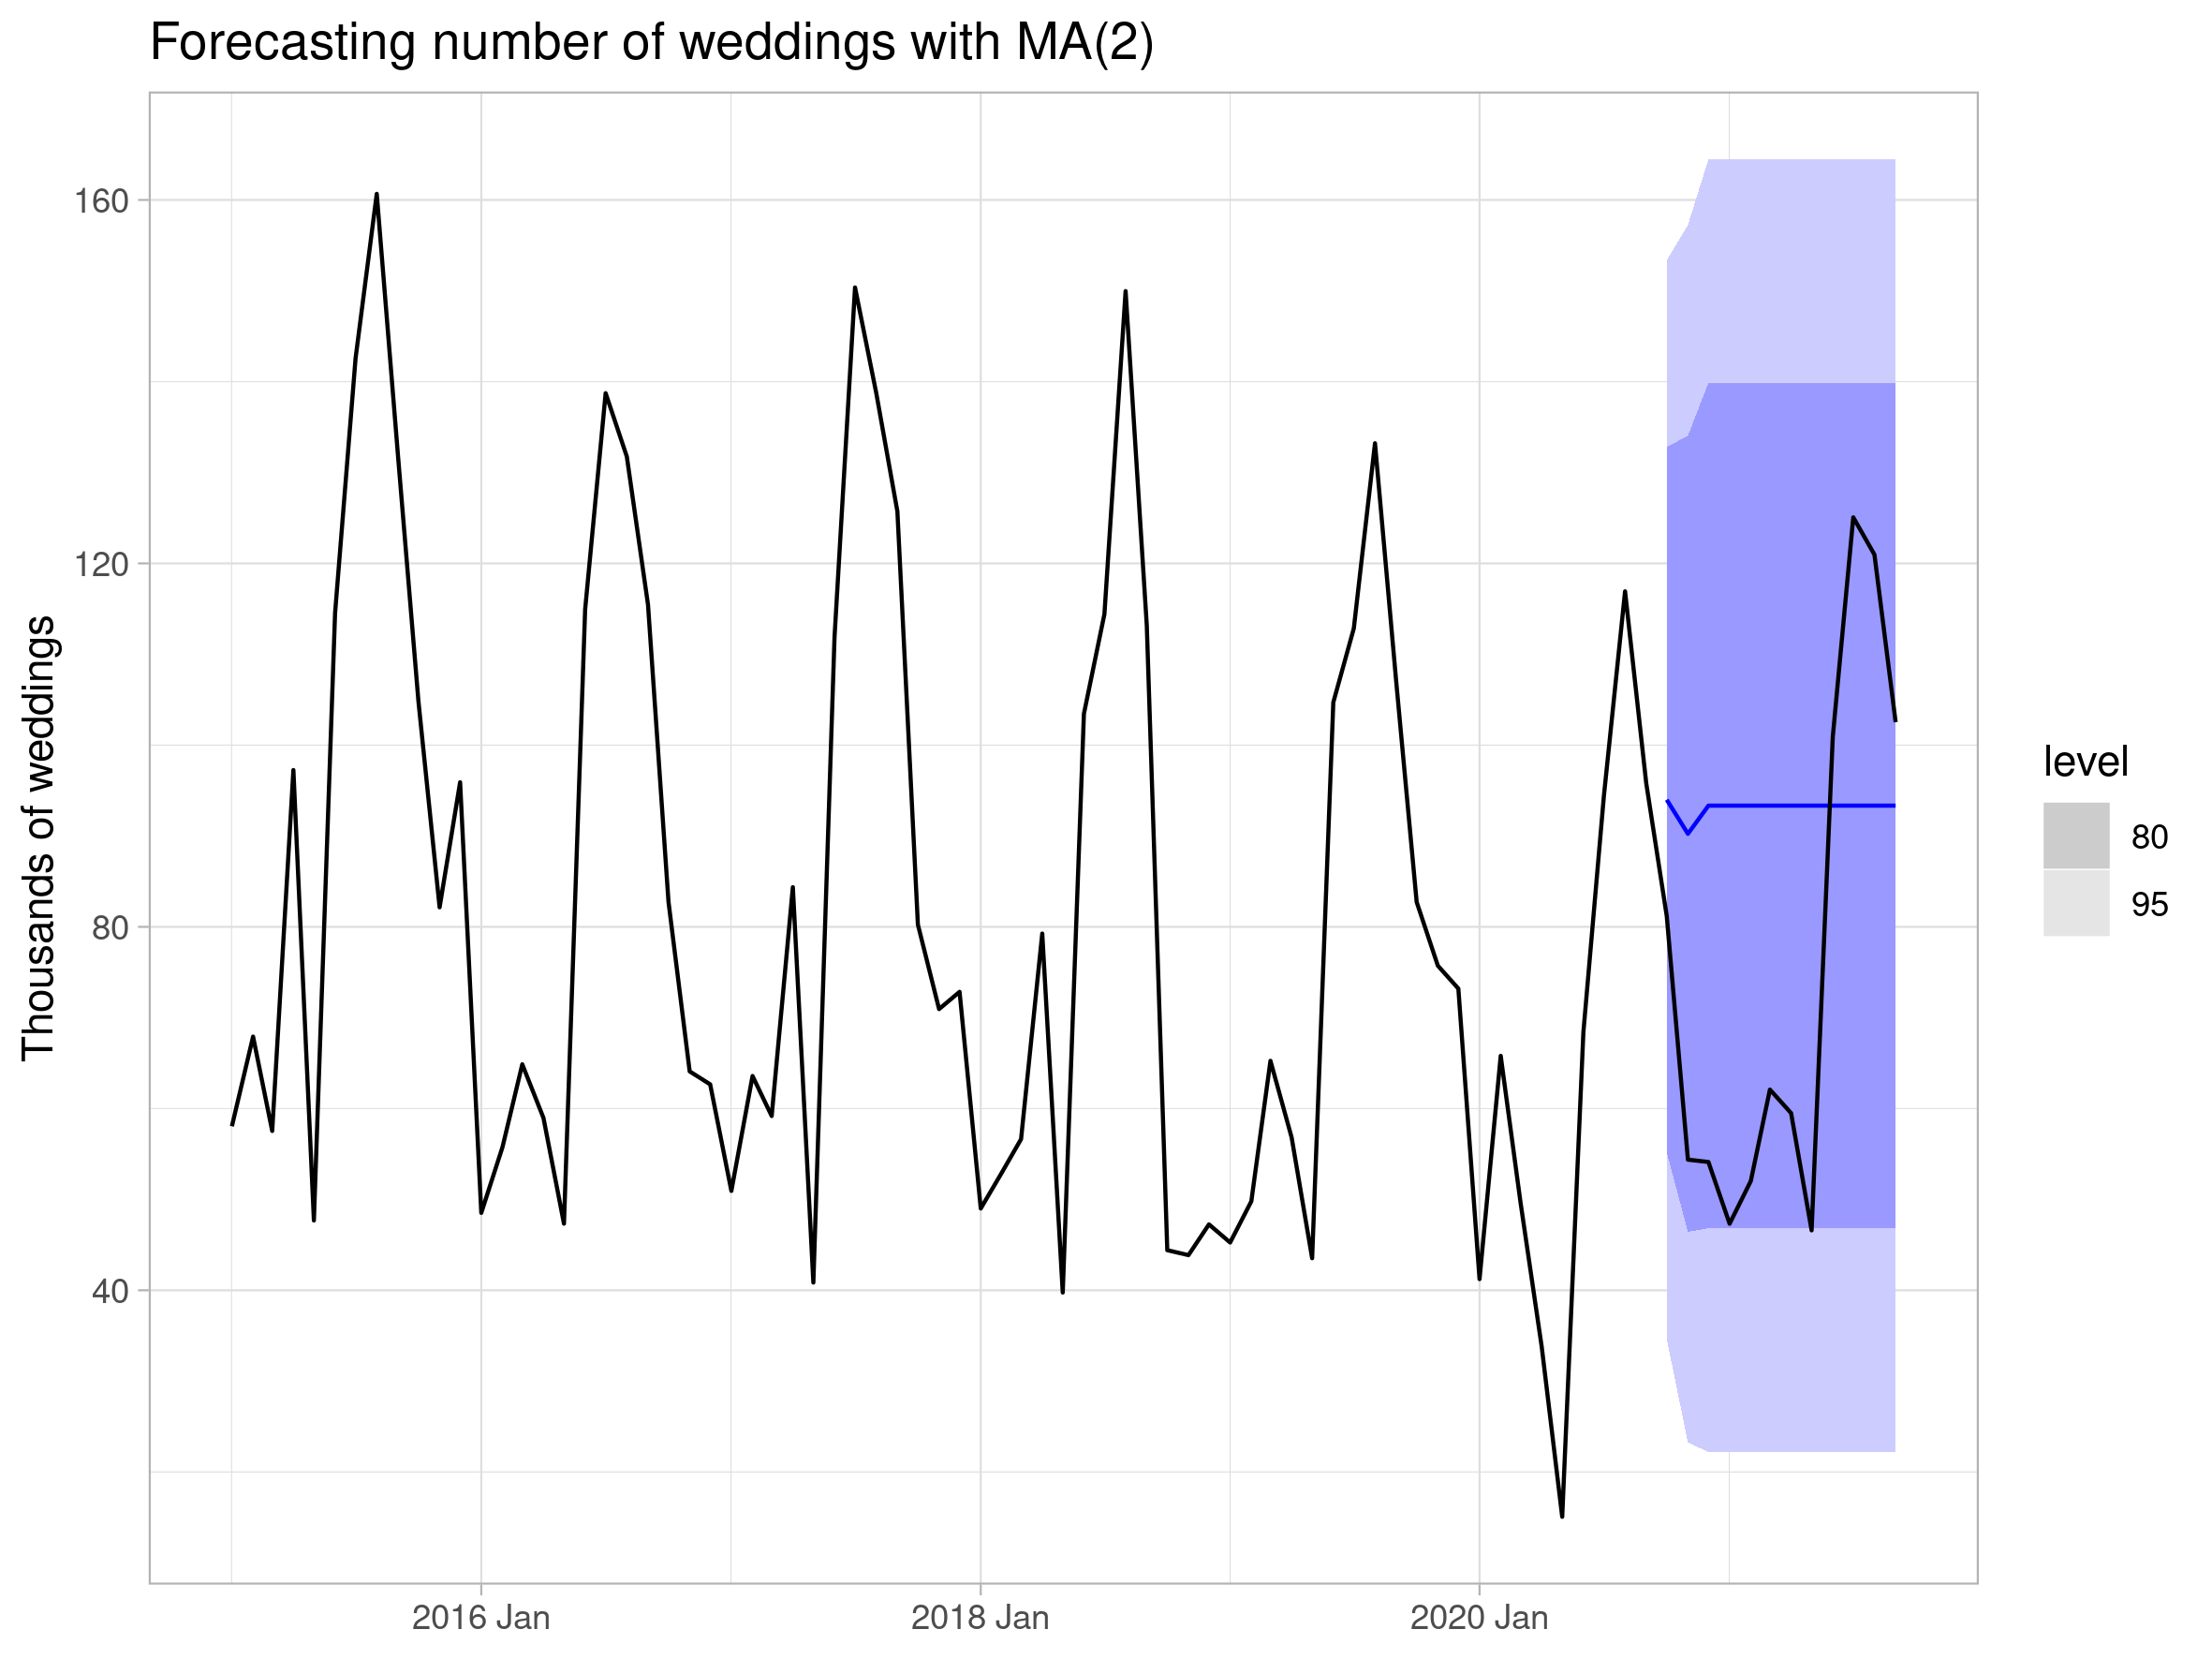
\includegraphics[width=\textwidth]{pictures/om_ts_04-094.png}
	
	
\end{frame}




\begin{frame}
	\frametitle{$MA(\infty)$}
	
	\begin{block}{Definition}
		Process $(y_t)$, which \alert{can} be represented as
		\[
		y_t = \mu + u_t + \alpha_1 u_{t-1} + \alpha_2 u_{t-2} + \ldots,
		\]
		where $(u_t)$ is white noise, an infinite number of $\alpha_i \neq 0$ and
		$\sum_{i=1}^{\infty} \alpha_i^2 < \infty$,
		is called the $MA(\infty)$ process
	\end{block}
	
	\pause
	$MA(\infty)$:
	\[
	y_t = 5 + u_t + 0.5 u_{t-1} + 0.5^2 u_{t-2} + 0.5^3 u_{t-3} + \ldots
	\]
	
	\pause
	And \alert{this is not allowed}:
	\[
	y_t = 5 + u_t + \frac{1}{\sqrt{2}}u_{t-1} + \frac{1}{\sqrt{3}} u_{t-2} + \frac{1}{ \sqrt{4}} u_{t-3} + \ldots
	\]
	
\end{frame}

\begin{frame}
	\frametitle{Convergences}
	\begin{block}{Theorem}
		If a
		$\sum_{i=0}^{\infty} \alpha_i^2 < \infty$ and $(u_t)$ is a zero-mean stationary process,
		then the sequence of partial sums $y^q_t$ of the form
		\[
		y^q_t = \mu + \sum_{i=0}^q \alpha_i u_{t-i}
		\]
		converges for $q \to \infty$ \alert{in mean}, \alert{in probability}, and \alert{in distribution}
	\end{block}
	
	Nuance: the convergence of the weighted sum is guaranteed for the stationary $(u_t)$
	\pause
	\begin{block}{Bonus}
		\ldots and the resulting process $(y_t)$ is stationary
	\end{block}
\end{frame}



\begin{frame}
	\frametitle{Wald's Theorem}
	
	\begin{block}{Theorem}
		If $(y_t)$ is a stationary process, then it can be represented as:
		\[
		y_t = \sum_{i=0}^{\infty} \alpha_i u_{t-i} + r_t,
		\]
		where
		\begin{itemize}
			\item $(u_t)$ — white noise,
			\item $\sum \alpha_i^2 < \infty$,
			\item $r_t$ is a linear \alert{predictable} random process,
			\item $\Cov(u_t, r_t) = 0$
		\end{itemize}
	\end{block}
	
	
\end{frame}

\begin{frame}
	\frametitle{Predictable Process}
	
	
	\begin{block}{Correct definition}
		A process $(r_t)$ is called \alert{linearly predictable} if
		\begin{itemize}
			\item $(r_t)$ is stationary,
			\item $r_t = \beta_0 + \beta_1 r_{t-1} + \beta_2 r_{t-2} + \ldots + \beta_p r_{t-p}$
		\end{itemize}
		
	\end{block}
	
\end{frame}




%\begin{frame}{$MA(\infty)$: summary}
%	
%	\begin{itemize}[<+->]
	%		\item \alert{Fast} coefficients tending to zero.
	%		\item \alert{Stationary process}.
	%		\item \alert{It's not clear yet how to evaluate.
		%		\end{itemize}
	%\end{frame}







\begin{frame}
	\frametitle{Reversibility condition}
	
	\begin{block}{Characteristic representation}
		The equation $MA(q)$ of the process satisfies the reversibility condition if
		the characteristic polynomial $\phi(\lambda)$ has all roots $\abs{\lambda_i} <1$
	\end{block}
	
	\pause
	
	\begin{block}{Lag representation}
		The equation $MA(q)$ of the process satisfies the reversibility condition if all roots  of 
		the lag polynomial $P(L)$ are  $\abs{\ell_i} >1$
	\end{block}
	
	
\end{frame}

\begin{frame}
	\frametitle{Example of reversible notation $MA(1)$}
	
	\[
	y_t = 5 + u_t + 0.5 u_{t-1}, \quad \sigma^2_u = 4
	\]
	\pause
	\[
	\lambda^1 + 0.5 \cdot \lambda^0
	\]
	\[
	\phi(\lambda) = \lambda + 0.5
	\]
	\pause
	\[
	\lambda_1 = -0.5
	\]
	
\end{frame}


\begin{frame}
	\frametitle{Example of $MA(1)$ irreversible notation}
	
	\[
	y_t = 5 + u_t + 2 u_{t-1}, \quad \sigma^2_u = 1
	\]
	\pause
	\[
	\lambda^1 + 2 \cdot \lambda^0
	\]
	\[
	\phi(\lambda) = \lambda + 2
	\]
	\pause
	\[
	\lambda_1 = -2
	\]
\end{frame}


\begin{frame}
	\frametitle{Nuance}
	
	\begin{block}{Difference}
		Stationarity is a property of the $(y_t)$ process itself.
		
		Reversibility is a property of the equation (process  notation) for~$(y_t)$.
	\end{block}
	
	\pause
    $MA(q)$ has a single notation when reversible
	
\end{frame}



\begin{frame}
\frametitle{MA process: Summary}
	
	\begin{itemize}[<+->]
		\item $MA(q)$ — weighting of several white noises
		\item $MA(q)$ is a stationary process
		\item $ACF$ vanishes sharply, $PACF$ tends to zero
 		\item Reversibility condition: roots of the characteristic polynomial $\abs{\lambda_i} < 1$ or 
		roots of the lag polynomial $\abs{\ell_i} > 1$.
	\end{itemize}
\end{frame}

% !TEX root = ../om_ts_002.tex

\begin{frame} % frame name
	
	\videotitle{ARMA equation}
	
\end{frame}



\begin{frame}{ARMA equation: Plan}
	\begin{itemize}[<+->]
		\item Definition
		\item Non-uniqueness of solutions
	\end{itemize}
		
\end{frame}

\begin{frame}
	\frametitle{About the purpose of old problems}
	
	Goal: A simple equation for a wide variety of processes
	
	\pause
	
	Problems:
	\begin{itemize}
		\item \alert{Non-uniqueness of equation} for one process
	\end{itemize}
	\pause
	
	Requirement: \alert{invertibility of the equation} \pause
	\begin{itemize}
		\item $MA(\infty)$ has \alert{infinite} number of parameters
	\end{itemize}
	
	\pause
	Let's try \alert{adding lags} $y_t$ to the equation!
	
	
\end{frame}


\begin{frame}
	\frametitle{New problem}
	
	\[
	y_t - y_{t-1} = u_t - u_{t-1}, \text{ where } (u_t) \text{ is white noise}
	\]
	
	\pause
	Solutions:
	\pause
	\begin{itemize}[<+->]
		\item $y_t = u_t$;
		\item $y_t = u_t - 0.7$;
		\item $y_t = u_t - 0.8$
	\end{itemize}
	
	\pause
	
	\alert{Infinite} number of solutions
	
\end{frame}


\begin{frame}
	\frametitle{ARMA equation}
	
	\begin{block}{Definition}
		Equation
		\[
		y_t = c + \beta_1 y_{t-1} + \ldots + \beta_p y_{t-p} + u_t + \alpha_1 u_{t-1} + \ldots + \alpha_q u_{t-q},
		\]
		where $(u_t)$ is white noise, we'll call an $ARMA$  equation
		
	\end{block}

	\alert{ARMA — Autoregression and Moving Average}	
	
	\pause
	\begin{block}{Definition}
		An equation of the form $P(L) y_t = c + Q(L) u_t$,
		where $(u_t)$ is white noise, $P(L)$ and $Q(L)$ are lag polynomials with $P(0)=Q(0)=1$, we'll call  an $ARMA$ equation
	\end{block}
	
\end{frame}

\begin{frame}
	\frametitle{ARMA equation: Summary}
	
	
	An equation is not a process! \pause 
	
	Why?
	

	\begin{itemize}[<+->]
		\item One equation has \alert{many solutions}
		\item One process can be described by \alert{several equations}
	\end{itemize}
	
\end{frame}



\begin{frame} % frame name
	
	\videotitle{ARMA process}
	
\end{frame}



\begin{frame}{ARMA process}
	\begin{itemize}[<+->]
		\item Equation irreducibility
		\item Solution structure
		\item ARMA process
	\end{itemize}
	
\end{frame}



\begin{frame}
	\frametitle{Irreducibility of Equation}
	
	\begin{block}{Definition}
		$ARMA$ an equation of the form $P(L) y_t = c + Q(L) u_t$ is called \alert{irreducible},
		if the polynomials $P(L)$ and $Q(L)$ do not have common roots
	\end{block}
	
	\pause
	Reducible Equation:
	\[
	y_t - y_{t-1} = u_t - u_{t-1} \text{ or } (1- L)y_t = (1 - L)u_t
	\]
	\pause
	Irreducible equation:
	\[
	y_t - y_{t-1} = u_t - 0.5u_{t-1} \text{ or } (1- L)y_t = (1 - 0.5L)u_t
	\]
	
\end{frame}





\begin{frame}
	\frametitle{Initial Conditions}
	Irreducible $ARMA$ equation:
	\[
	y_t = 0.5 y_{t-1} + u_t, \text{ where } (u_t) \text{ is white noise}
	\]
	
	\pause
	Let's try different initial conditions:
	\pause
	\begin{itemize}
		\item $\alert{y_0=0}$
	\end{itemize}
	\pause
	$y_1 = u_1$, $y_2 = u_2 + 0.5 u_1$, $y_3 = u_3 + 0.5 u_2 + 0.25 u_1$, \ldots
	\pause \pause
	\begin{itemize}
		\item $\alert{y_0=2u_1}$
	\end{itemize}
	\pause
	$y_1 = 2u_1$, $y_2 = u_2 + u_1$, $y_3 = u_3 + 0.5 u_2 + 0.5 u_1$, \ldots
	\pause
	
	The initial conditions also determine the past $y_t$!
	
\end{frame}

\begin{frame}
	\frametitle{ARMA Solutions}
	
	\begin{block}{Theorem I}
		Any $ARMA$ equation with at least one $y_t$ lag has an infinite number of solutions
	\end{block}
	
	\pause
	\begin{block}{Theorem II}
		In order to obtain a unique solution of an $ARMA$  equation of the form $P(L)y_t = c + Q(L) u_t$,
		it suffices to specify the initial conditions in an amount equal to the power of $P(L)$
	\end{block}
	\pause
	\[
	y_t = 0.6 y_{t-1} + 0.08y_{t-2} + u_t \pause \text{ and } \alert{y_0 = u_0, y_1 = u_0 + 4}
	\]
	
\end{frame}

\begin{frame}
	\frametitle{And how many stationary solutions?}
	
	\begin{block}{Correct theorem}
		If an $ARMA$ equation $P(L) y_t = c + Q(L) u_t$ is irreducible, then it
		\begin{itemize}
			\item has exactly one stationary solution if the lag polynomial $P(\ell)$ has all roots $\abs{\ell_i} \neq 1$;
			\item has no stationary solutions if the lag polynomial $P(\ell)$ has a root with $\abs{\ell_i} = 1$
		\end{itemize}
	\end{block}
	
	\pause
	\begin{itemize}
		\item $y_t = 0.5 y_{t-1} + u_t, P(L) = 1 - 0.5L, \ell_1 = 2$: \pause one stationary solution;
	\end{itemize}
	\pause
	\begin{itemize}
		\item $y_t = y_{t-1} + u_t, P(L) = 1 - L, \ell_1 = 1$: no stationary solutions
	\end{itemize}
	
\end{frame}



\begin{frame}
	\frametitle{AR process}
	
	\begin{block}{Definition}
		$AR(p)$ process with equation
		\[
		y_t = c + \beta_1 y_{t-1} + \ldots + \beta_p y_{t-p} + u_t,
		\]
		where $(u_t)$ is white noise and $\beta_p \neq 0$, is the
		solution of this equation in  the form of $MA(\infty)$ with respect to $(u_t)$
	\end{block}
	
	\pause
	\begin{block}{Definition with lags}
		$AR(p)$ process with equation
		\[
		P(L)y_t = c + u_t,
		\]
		where $(u_t)$ is white noise, $P(L)$ has power $p$ and $P(0)=1$, is the 
		solution of this equation in the form of $MA(\infty)$ with respect to~$(u_t)$
	\end{block}
	
\end{frame}

\begin{frame}
	\frametitle{Definitions by different authors}
	


	In our definition of $AR(p)$, the process is necessarily \alert{stationary}.
	
	\pause
	Some  authors \alert{do not include}  the requirement of stationarity in the definition of $AR(p)$.
	
\end{frame}

\begin{frame}
	\frametitle{ARMA process}
	
	\begin{block}{Definition}
		$ARMA(p, q)$ process with equation
		\[
		y_t = c + \beta_1 y_{t-1} + \ldots + \beta_p y_{t-p} + u_t + \alpha_1 u_{t-1} + \ldots + \alpha_q u_{t-q},
		\]
		where $(u_t)$ is white noise, $\beta_p \neq 0$, $\alpha_q \neq 0$ and the equation is irreducible, is the
		solution of this equation in the form of $MA(\infty)$ with respect to $(u_t)$
	\end{block}
	
	\pause
	\begin{block}{Definition with lags}
		$ARMA(p,q)$ process with equation
		\[
		P(L)y_t = c + Q(L)u_t,
		\]
		where $(u_t)$ is white noise, $P(L)$ and $Q(L)$ have powers $p$ and $q$, respectively, are irreducible and $P(0)=Q(0)=1$, is 	the solution of this equation in  the form $MA(\infty)$ with respect to $(u_t)$
	\end{block}
\end{frame}


\begin{frame}
	\frametitle{What about non-uniqueness?}
	
	The same $ARMA(p, q)$ process $(y_t)$ can be described by different equations!
	\pause
	
	\begin{block}{Invertibility}
		If the series $(y_t)$ is an $ARMA(p, q)$ process with the equation $P(L) y_t = c + Q(L) u_t$,
		then this equation will be unique if the $MA$ part satisfies the invertibility condition.
	\end{block}
	
	\pause
	Condition for  invertibility of the $ARMA$ equation:
	\begin{itemize}
		\item the characteristic polynomial $\phi_{MA}(\lambda)$ has all roots $\abs{\lambda_i} <1$;
		\item the lag polynomial $Q(L)$ has all roots $\abs{\ell_i} >1$
	\end{itemize}
	
	
\end{frame}



\begin{frame}
	\frametitle{ARMA process: Summary}
	\begin{itemize}[<+->]
		\item The process is stationary by \alert{definition}
		\item $AR$ and $MA$ processes are \alert{special cases} of the $ARMA$ process
		\item Theoretical $ACF$ and $PACF$ decrease \alert{exponentially}
		\item The invertibility condition guarantees \alert{uniqueness}
		\item An irreducible equation either has a \alert{unique} stationary solution  or it does not exist
	\end{itemize}
\end{frame}
% !TEX root = ../om_ts_002.tex

\begin{frame} % название фрагмента

\videotitle{ARIMA process}

\end{frame}



\begin{frame}{ARIMA process: Plan}
  \begin{itemize}[<+->]
	\item Stationarity of $ARMA$
	\item Definition of $ARIMA$
	\item Differencing
  \end{itemize}

\end{frame}



\begin{frame}
	\frametitle{Nuances}
	
	\begin{itemize}
		\onslide<1->{\item Process $y_t \sim ARMA(p, q)$ is stationary \alert{by definition}:}
		
		\onslide<2->{$\E(y_t) = \mu_y$, $\Var(y_t) = \gamma_0$, $\Cov(y_t, y_{t-k}) = \gamma_k$}
		
		\onslide<3->{\item In the \alert{canonical notation} $ARMA(p, q)$ of the process $P(L) y_t = c+ Q(L) u_t$ for the polynomial $P(L)$
			all roots $\abs{\ell} > 1$}
				
		\onslide<4->{\item When estimating the $ARMA(p, q)$ process by the maximum likelihood method, these restrictions are imposed \alert{a priori}}
		
	\end{itemize}
	
\end{frame}


\begin{frame}
	\frametitle{What to do with non-stationary processes?}
	
	\begin{block}{Definition}
		The random process $(y_t)$ is called the $ARIMA(p, 1, q)$ w.r.t. the white noise process $(u_t)$,
		if $(y_t)$ is non-stationary, but $\Delta y_t$ is a stationary $ARMA(p, q)$ process w.r.t. the  white noise $(u_t)$
	\end{block}
	
	\pause
	
	\begin{block}{Definition}
		The random process $(y_t)$ is called the $ARIMA(p, 2, q)$ w.r.t. the  white noise process $(u_t)$,
		if $(y_t)$ and $(\Delta y_t)$ are non-stationary, but $\Delta^2 y_t$ is a stationary $ARMA(p, q)$ process w.r.t. the white noise $(u_t)$
	\end{block}
	
	\pause
	$\Delta y_t = y_t - y_{t-1}$ and $\Delta^2 y_t = \Delta y_t - \Delta y_{t-1}$
	
	\pause
	ARIMA — \alert{A}uto\alert{R}egressive \alert{I}ntegrated \alert{M}oving \alert{A}verage
	
\end{frame}

\begin{frame}
	\frametitle{How to choose?}
	
	$ARIMA(p, 0, q)$ or $ARIMA(p, 1, q)$ or $ARIMA(p, 2, q)$
	\begin{itemize}
		\onslide<2->{\item Analyse the \alert{graph}:}
		\onslide<3->{stationary process graph oscillates around its mean with a \alert{constant deviation}}
		
		\onslide<4->{\item Evaluate all the models and choose the best one by \alert{cross-validation}}
		\onslide<5->{Time consuming!}
		
		\onslide<6->{\item \alert{You cannot use $AIC$}!}
		
		\onslide<7->{$\ln L(y_1, \ldots, y_n \mid \theta)$ and $\ln L(y_2, \ldots, y_n \mid \theta, y_1)$ and $\ln L( y_3, \ldots, y_n \mid \theta, y_1, y_2)$
			incomparable!}
		\onslide<8->{\item There are \alert{unit root tests}!}
		
		\onslide<9->{ADF, KPSS, PP, \ldots}
	\end{itemize}
	
\end{frame}

\begin{frame}
	\frametitle{Analysing the graphs}
	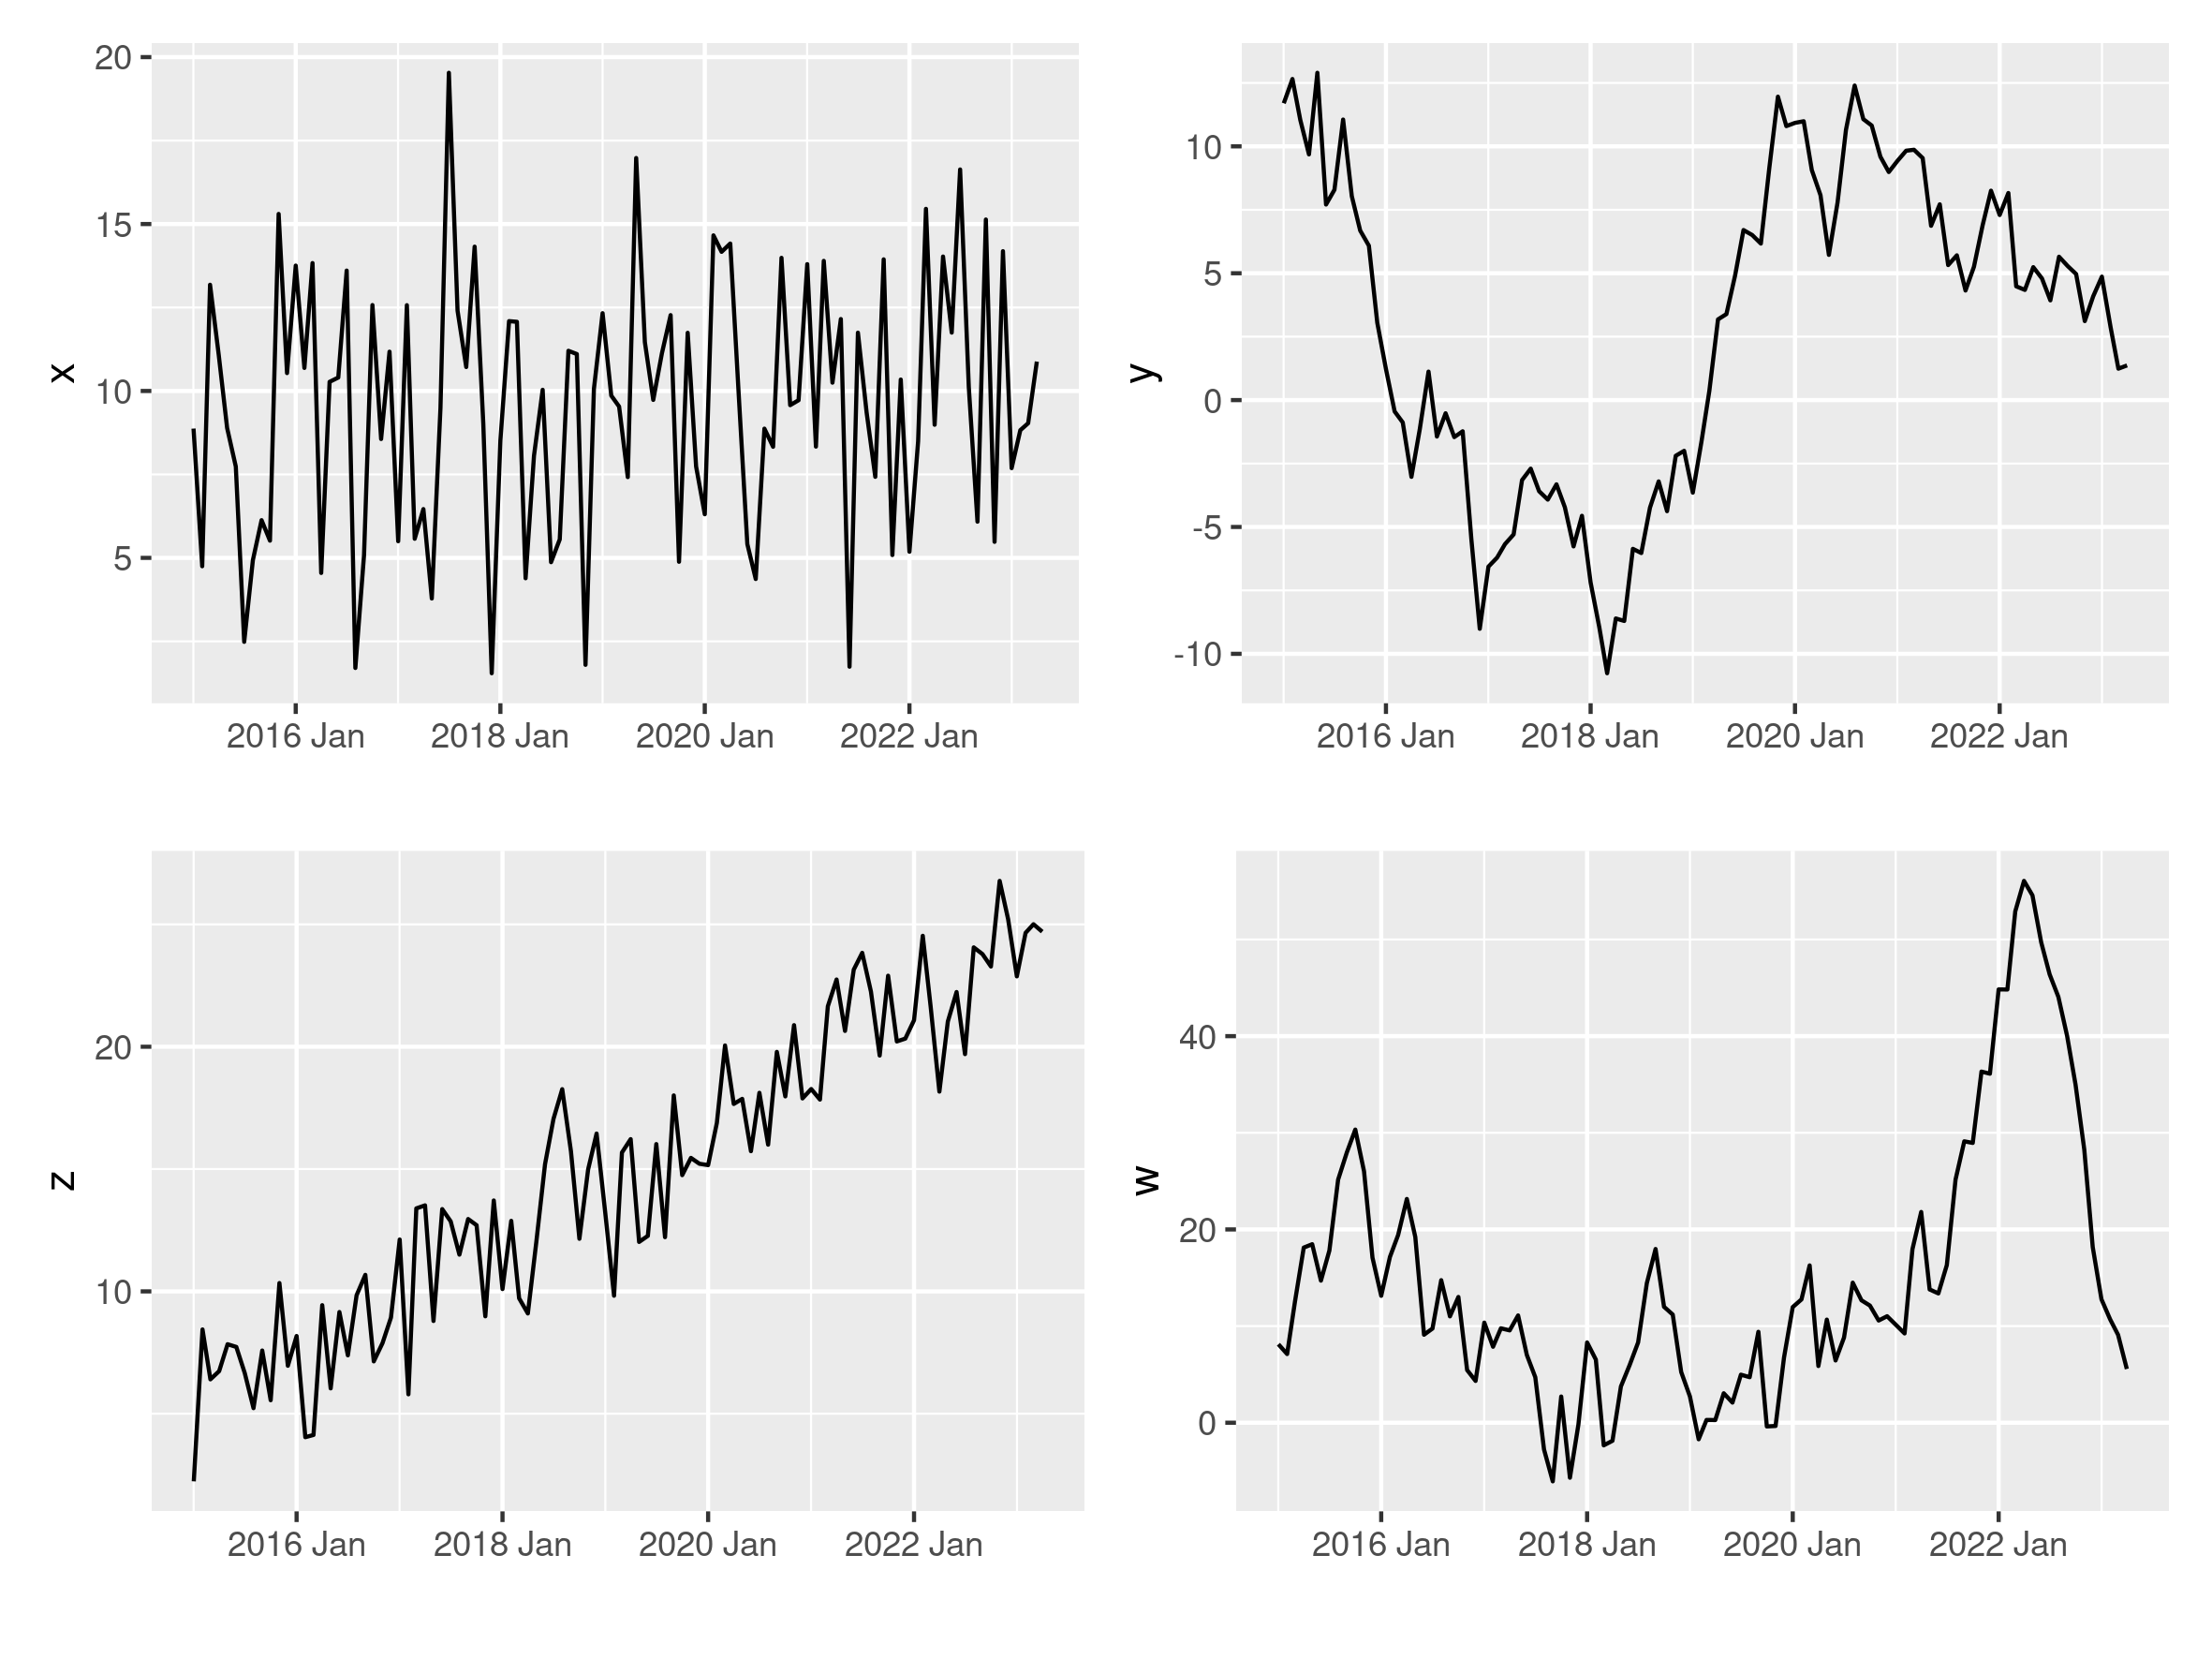
\includegraphics[width=\textwidth]{pictures/om_ts_06-027.png}
\end{frame}


\begin{frame}{ARIMA: Summary}
	
	\begin{itemize}[<+->]
		\item $ARMA$ is for \alert{stationary} series
		\item Sometimes $\Delta y_t$ or $\Delta^2 y_t$ is stationary
		\item Choose between $ARMA$ and $ARIMA$
	\end{itemize}
\end{frame}


\begin{frame} % название фрагмента
	
	\videotitle{SARIMA process}
	
\end{frame}



\begin{frame}{SARIMA process: Plan}
	\begin{itemize}[<+->]
		\item Seasonal $ARMA$

		\item Seasonal $ARIMA$
		
		\item Choosing between models
	\end{itemize}
	
\end{frame}


\begin{frame}
	\frametitle{Seasonality and $ARIMA$}
	
	Using $ARMA$ and $ARIMA$ models, we can model seasonality!
	
	\pause
	\[
	MA(12): y_t = c + u_t + a_1 u_{t-1} + a_2 u_{t-2} + \ldots + a_{12} u_{t-12}.
	\]
	\[
	ARIMA(12, 1, 0): \Delta y_t = c + u_t + b_1 \Delta y_{t-1} + \ldots + b_{12} \Delta y_{t-12}.
	\]
	
\end{frame}



\begin{frame}
	\frametitle{ARMA should be economical!}
	
	Let's focus on \alert{non-zero} coefficients!
	\pause
	\begin{block}{Definition}
		If the stationary $ARMA$ model for $y_t$ can be written with fewer parameters as
		\[
		P_{non}(L)P_{seas}(L^{12}) y_t = c + Q_{non}(L) Q_{seas}(L^{12}) u_t,
		\]
		where the degrees of the lag polynomials are $\deg P_{non} =p$, $\deg P_{seas} =P$, $\deg Q_{non} =q$, $\deg Q_{seas} =Q$,
		then it is also called $SARMA(p, q)(P, Q)[12]$
	\end{block}
\end{frame}


\begin{frame}
	\frametitle{Examples}
	
	\begin{itemize}
		\item $SARMA(\alert{1},0)(0,\alert{2})[12]$
	\end{itemize}
	
	
		\[
		(1 - b_{\alert{1}} L) y_t = c + (1 + d_1 L^{12} + d_{\alert{2}} L^{24}) u_t;
		\]
	
	\pause 
		
	\begin{itemize}
		
		\item $SARMA(0,\alert{2})(\alert{1},0)[12]$
	\end{itemize}		

		\[
(1 - f_{\alert{1}} L^{12}) y_t = c + (1 + a_1 L + a_{\alert{2}} L^2) u_t;
\]

		
	\pause 
		
	\begin{itemize}
		
		\item $SARMA(\alert{1},\alert{2})(2,1)[12]$
	\end{itemize}



		\[
		(1 - f_1 L^{12} - f_{\alert{2}} L^{24}) (1 - b_{\alert{1}} L^1) y_t = c + (1 + a_1 L + a_2 L^2) (1 + d_1 L^{12}) u_t
		\]
	
	
	
\end{frame}





\begin{frame}
	\frametitle{SARIMA}
	
	By analogy with the difference $\Delta y_t = y_t - y_{t-1}$, we can consider the seasonal difference $\Delta_{12} y_t = y_t - y_{t-12}$
	
	\pause
	\begin{block}{Definition}
		If the series $z_t = \Delta^{\alert{d}} \Delta^{\alert{D}}_{12} y_t$ is described by the stationary model $SARMA(p, q)(P, Q)[12]$ ,
		then $y_t$ is said to be described by the $SARIMA(p, \alert{d}, q)(P, \alert{D}, Q)[12]$ model
	\end{block}
	\pause
	$d$ is the number of times the first difference should be taken $\Delta = 1 - L$;
	
	$D$ is the number of times the seasonal  difference should be taken $\Delta_{12} = 1- L^{12}$;
	\pause
	$y_t \sim SARIMA(0, 0, 2)(1, \alert{1}, 2)[12]$ means that
	
	$\Delta_{12} y_t \sim SARMA(0, 2)(1, 2)[12]$
\end{frame}

\begin{frame}
	\frametitle{How to choose?}
	
	$SARIMA(p, 0, q)(P, 0, Q)$ or $SARIMA(p, 0, q)(P, 1, Q)[12]$?
	
	\begin{itemize}
		\onslide<2->{\item Analyse the \alert{graph}!}
				
		\onslide<3->{\item Evaluate all these models and choose the best one by \alert{cross-validation}}
		\onslide<4->{Time consuming!}
		
		\onslide<5->{\item \alert{You cannot use $AIC$}!}
		\onslide<6->{The conditional and unconditional likelihood functions contain different numbers of terms.}
		
		\onslide<7->{\item There are \alert{unit root tests}!}
		
		\onslide<8->{And rules of thumb\ldots}
	\end{itemize}
	
\end{frame}


\begin{frame}
	\frametitle{STL decomposition and the power of seasonality}
	
	\onslide<1->{Step 1. Find the $STL$ expansion of the series $(y_t)$
		\[
		y_t = trend_t + seas_t + remainder_t
		\]}
	
	\onslide<2->{Step 2. Calculate the strength of seasonality
		\[
		F_{seas} = \max\left\{1 - \frac{\sVar(remainder)}{\sVar(seas + remainder)}, 0 \right\}
		\]}
	
	\onslide<3->{Step 3. If the strength of seasonality is above the threshold, then move to $\Delta_{12} y_t = y_t - y_{t-12}$}
	
\end{frame}



\begin{frame}{SARIMA: Summary}
	
	\begin{itemize}[<+->]
		\item Seasonal ARIMA is more compact
		\item The strength of seasonality from the \alert{STL} expansion is used to decide if a seasonal difference $\Delta_{12} y_t$ is needed

	\end{itemize}
\end{frame}


% !TEX root = ../om_ts_002.tex


\begin{frame} % frame name
	
	\videotitle{Unit root tests: ADF test}
	
\end{frame}




\begin{frame}{ADF test: Plan}
	\begin{itemize}[<+->]
		\item Test assumptions
		\item Test algorithm
		\item Three variations of the test
	\end{itemize}
	
\end{frame}




\begin{frame}
	\frametitle{Why do we need an stationarity tests?}
	
	We want to answer the questions:
	\pause
	\begin{itemize}[<+->]
		\item Should the $ARMA$ model be used for $(y_t)$ or for $(\Delta y_t)$?
		\item How to include a constant in a model?
	\end{itemize}
	
	\pause
	Name "unit root test":
	\pause
	\[
	\Delta = 1 - L = P(L)
	\]
	The equation $1 - \ell = 0$ has a root $\ell =1$
	
\end{frame}


\begin{frame}
	\frametitle{ADF test}
	
	ADF — \alert{Augmented Dickey Fuller} test
	
	\pause
	Three variations of the test: without a constant, with a constant, with a trend
	
\end{frame}


\begin{frame}
	\frametitle{ADF with constant}
	\[
	\Delta y_t = c + \beta y_{t-1} + d_1 \Delta y_{t-1} + \ldots + d_p \Delta y_{t-p} + u_t,
	\]
	
	\pause
	
	\alert{$H_0$: $\beta = 0$}
	
	$\Delta y_t = m + x_t$;
	
	$(x_t)$ is a stationary $AR(p)$ process with $\E(x_t) = 0$;
	
	$y_t = y_0 + mt + \sum_{i=1}^t x_i$
	
	\pause
	
	\alert{$H_a$: $\beta < 0$}
	
	$(y_t)$ is a stationary $AR(p + 1)$ process
	
\end{frame}

\begin{frame}
	\frametitle{ADF with constant: $H_0$ and $H_a$}
	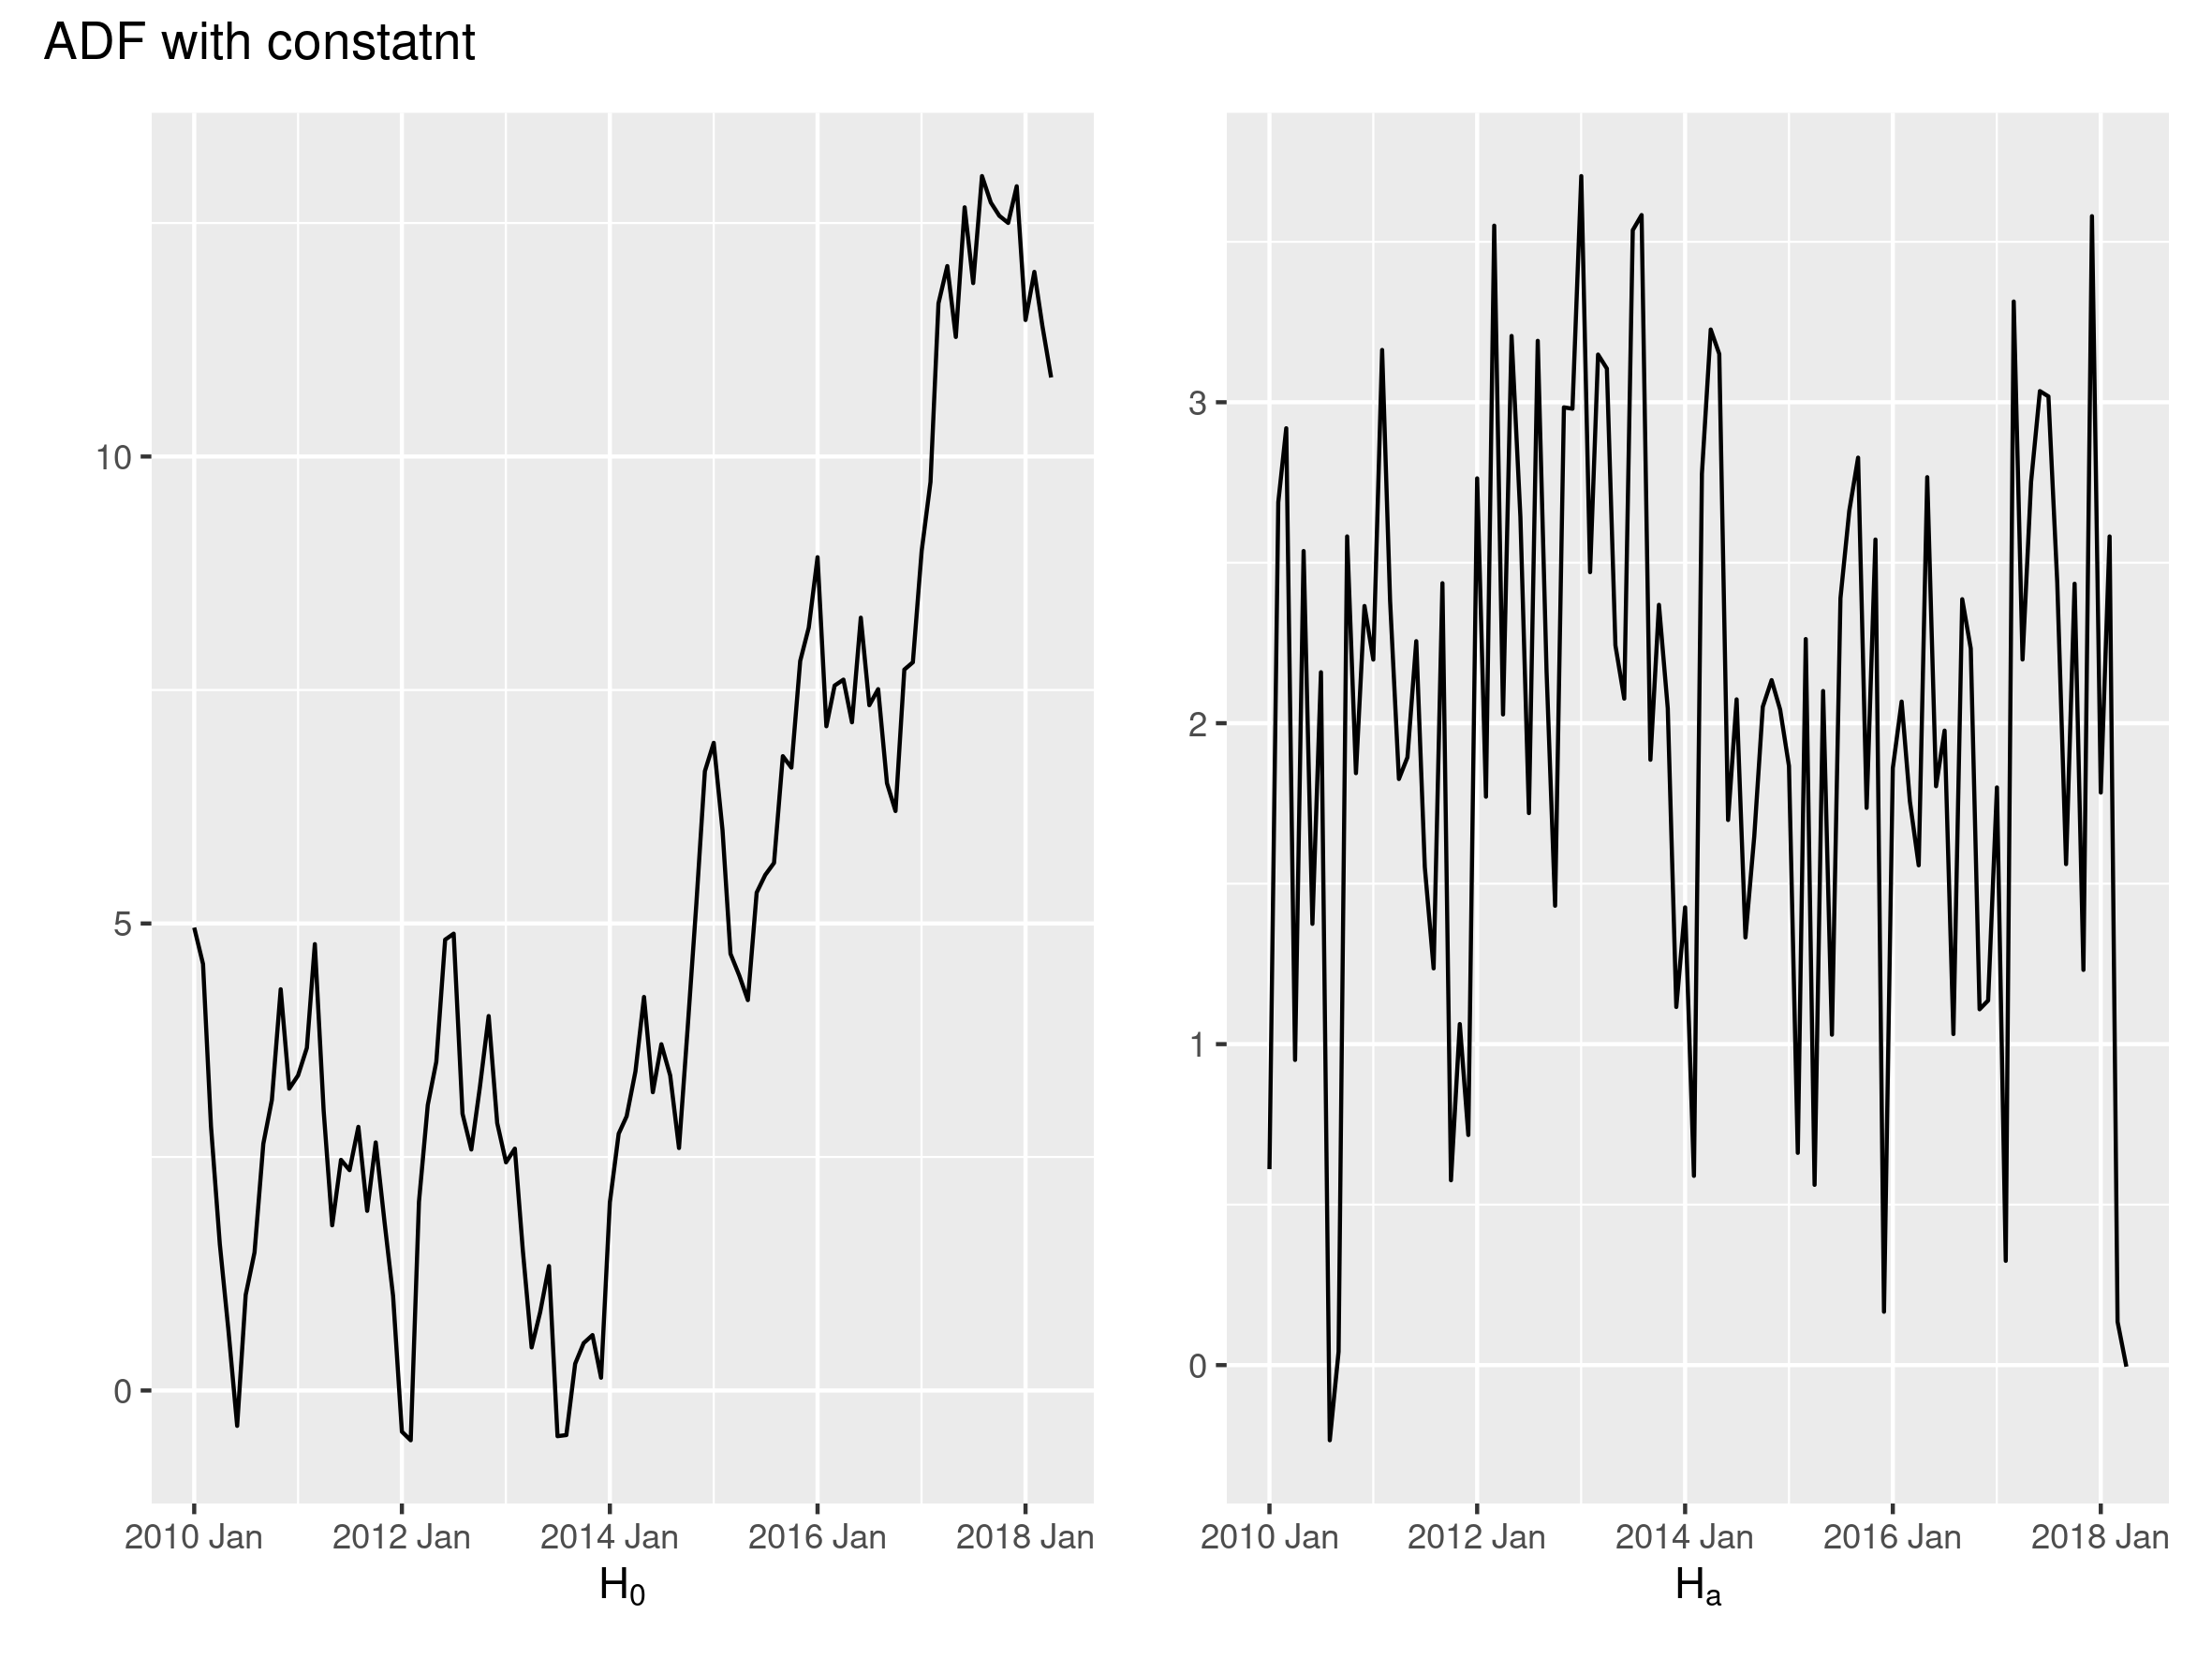
\includegraphics[width=\textwidth]{pictures/om_ts_06-046.png}
	
\end{frame}

\begin{frame}
	\frametitle{ADF with constant: algorithm}
	
	Step 1. Evaluate \alert{regression}
	\[
	\widehat{\Delta y_t} = \hat c + \hat \beta y_{t-1} + \hat d_1 \Delta y_{t-1} + \ldots + \hat d_p \Delta y_{t-p}
	\]
	
	\pause
	Step 2. Calculate the $t$-statistics using the \alert{classic formula}
	\[
	ADF = \frac{\hat \beta - 0}{se(\hat \beta)}
	\]
	
	\pause
	Under true $H_0$, the distribution of the $ADF$-statistic converges to the  special  \alert{DF distribution} with $DF^c$!
	
	\pause
	Step 3. We conclude:
	
	If $ADF < DF^c$ then $H_0$ is rejected
	
\end{frame}


\begin{frame}
	\frametitle{ADF without constant}
	\[
	\Delta y_t = \beta y_{t-1} + d_1 \Delta y_{t-1} + \ldots + d_p \Delta y_{t-p} + u_t,
	\]
	
	\pause
	
	\alert{$H_0$: $\beta = 0$}
	
	$(\Delta y_t)$ is a stationary $AR(p)$ process with $\E(\Delta y_t) = 0$;
	
	$y_t = y_0 + \sum_{i=1}^t \Delta y_i $
	
	\pause
	
	\alert{$H_a$: $\beta < 0$}
	
	$(y_t)$ is a stationary $AR(p + 1)$ process with $\E(y_t) = 0$;
	
	\pause
	
	The algorithm will have \alert{regression without a constant} and another distribution $DF^0$
	
\end{frame}


\begin{frame}
	\frametitle{ADF without constant: $H_0$ and $H_a$}
	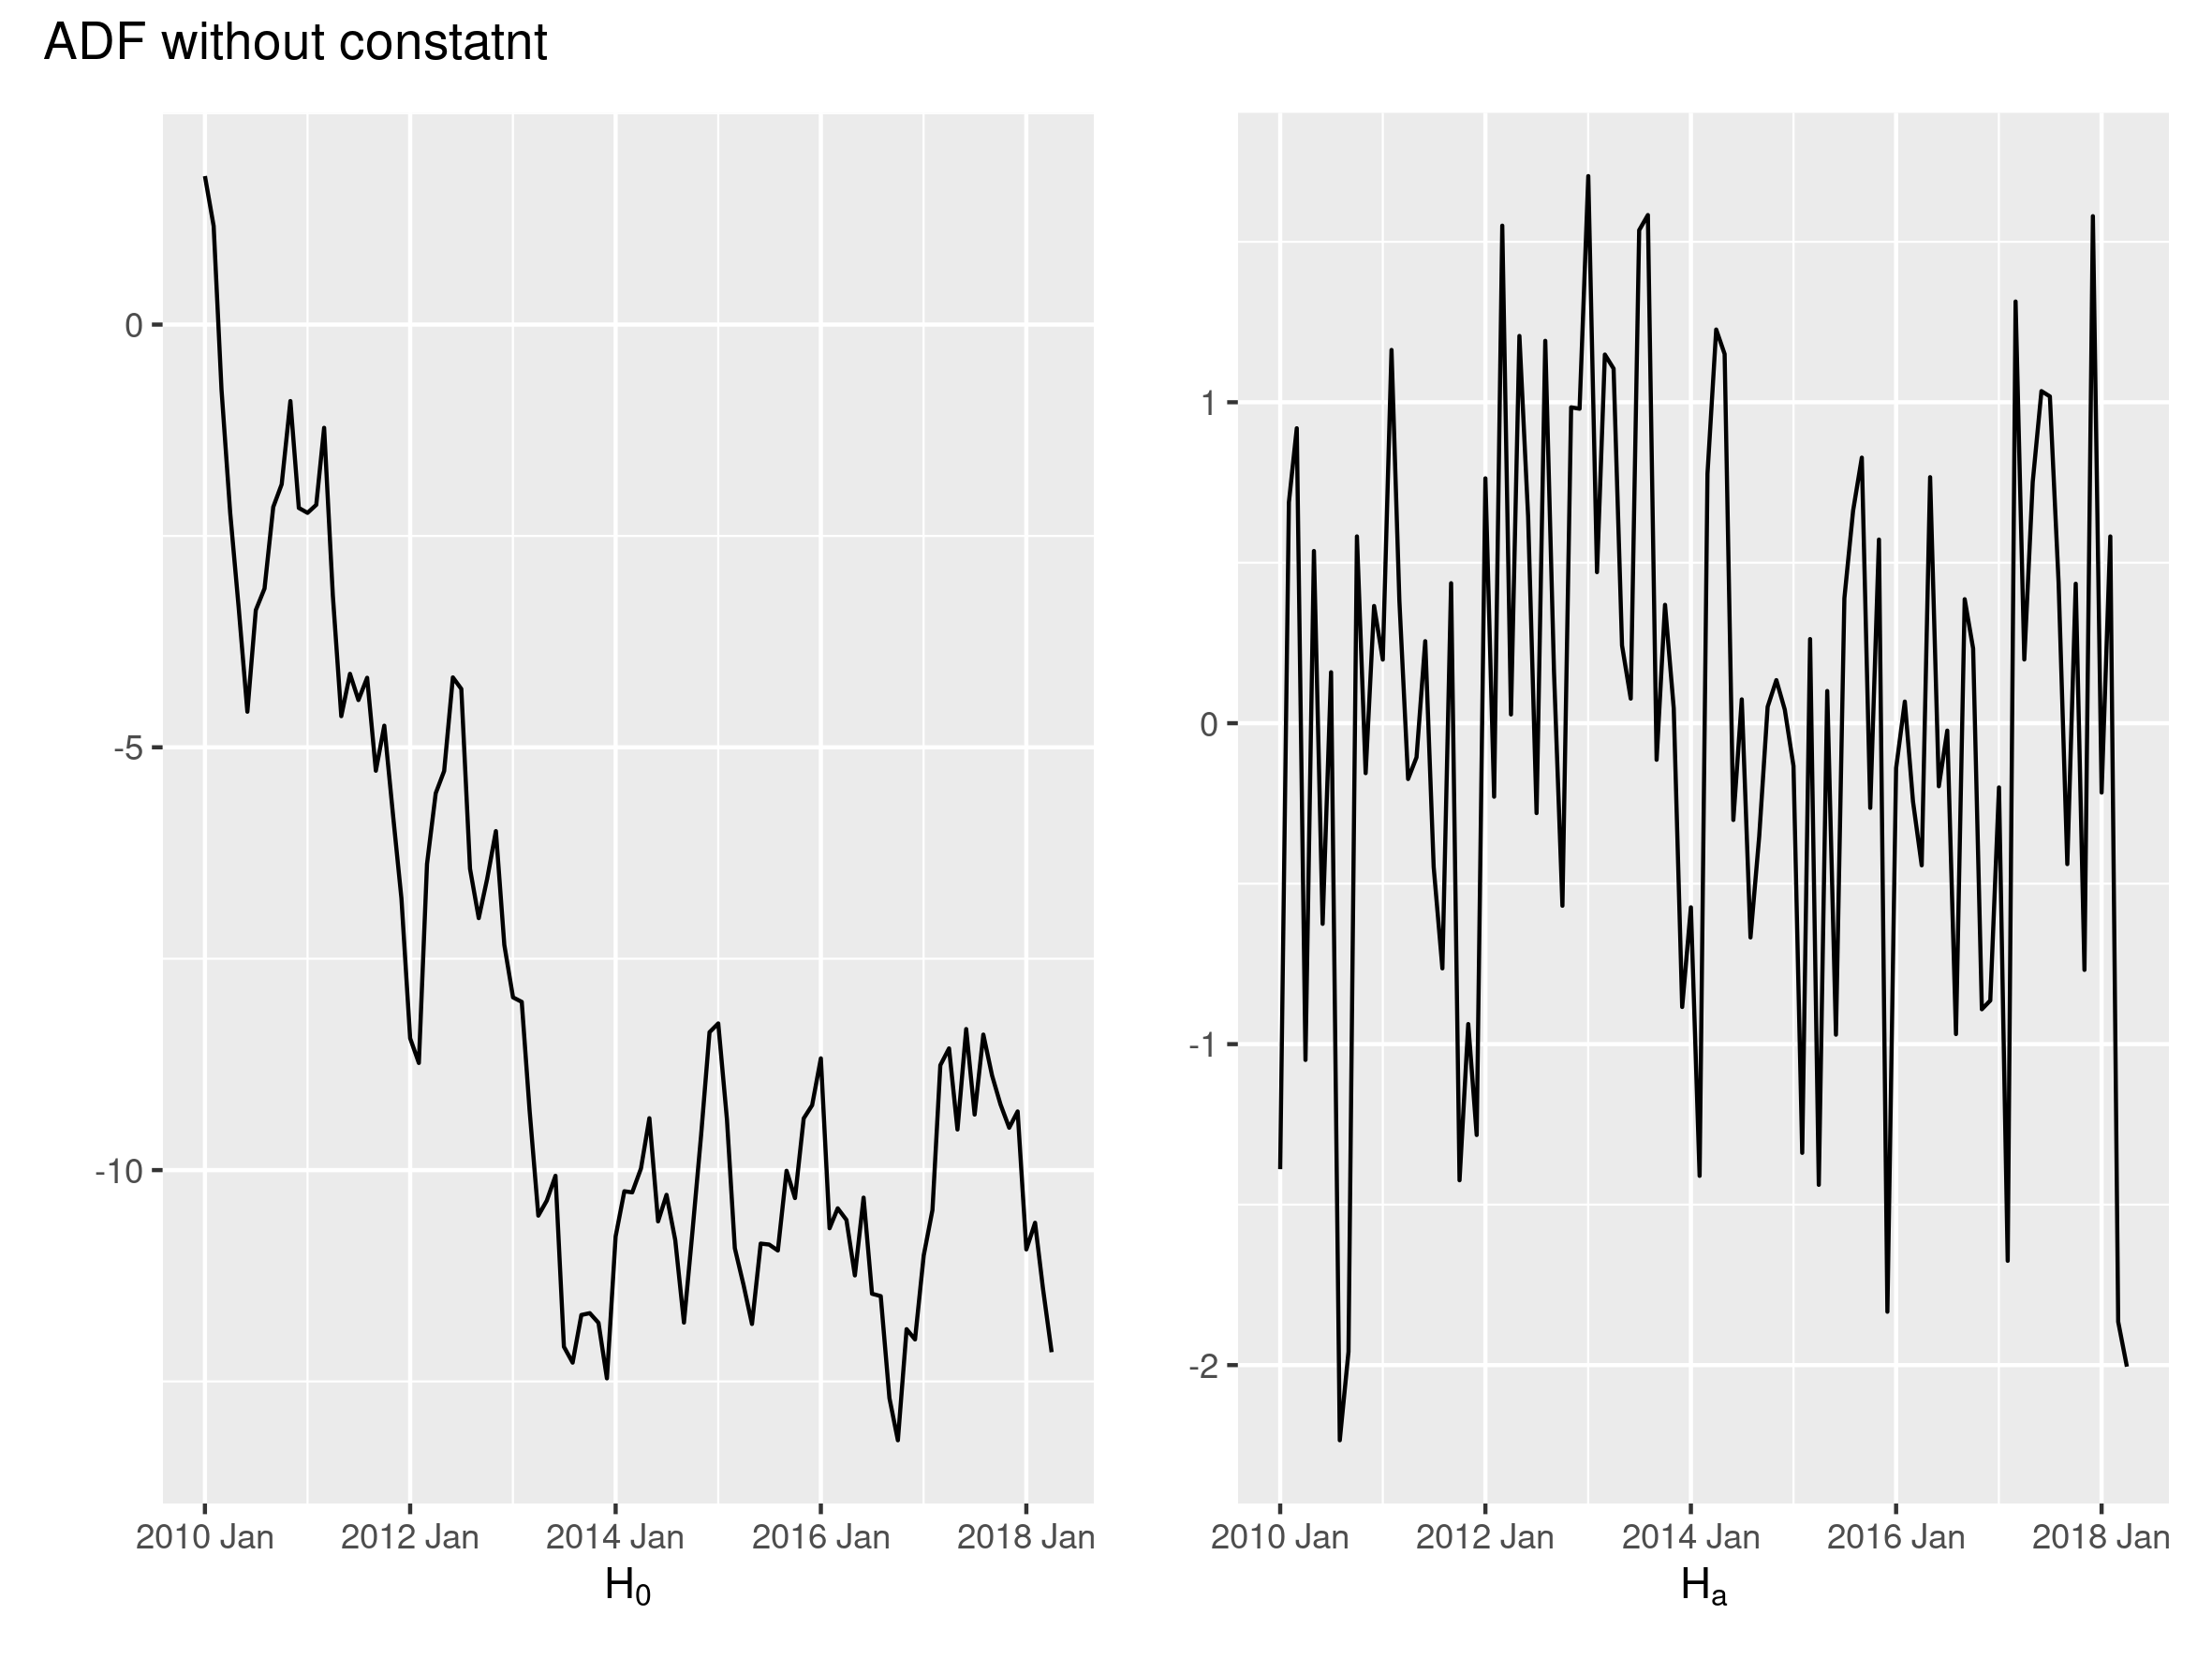
\includegraphics[width=\textwidth]{pictures/om_ts_06-055.png}
	
\end{frame}



\begin{frame}
	\frametitle{ADF with trend}
	\[
	\Delta y_t = c + g t + \beta y_{t-1} + d_1 \Delta y_{t-1} + \ldots + d_p \Delta y_{t-p} + u_t,
	\]
	
	\pause
	
	\alert{$H_0$: $\beta = 0$}
	
	$\Delta y_t = k_1 + k_2t + x_t$;
	
	$(x_t)$ is a stationary $AR(p)$ process with $\E(x_t) = 0$;
	
	$y_t = y_0 + m_1 t + m_2 t^2 + \sum_{i=1}^t x_i$
	
	\pause
	
	\alert{$H_a$: $\beta < 0$}
	
	$y_t = m_1 + m_2t + x_t$;
	
	$(x_t)$ is a stationary $AR(p + 1)$ process with $\E(x_t) = 0$;
	
	\pause
	
	The algorithm will have a regression \alert{with a constant and a trend} and another distribution $DF^{ct}$
	
\end{frame}


\begin{frame}
	\frametitle{ADF with trend: $H_0$ and $H_a$}
	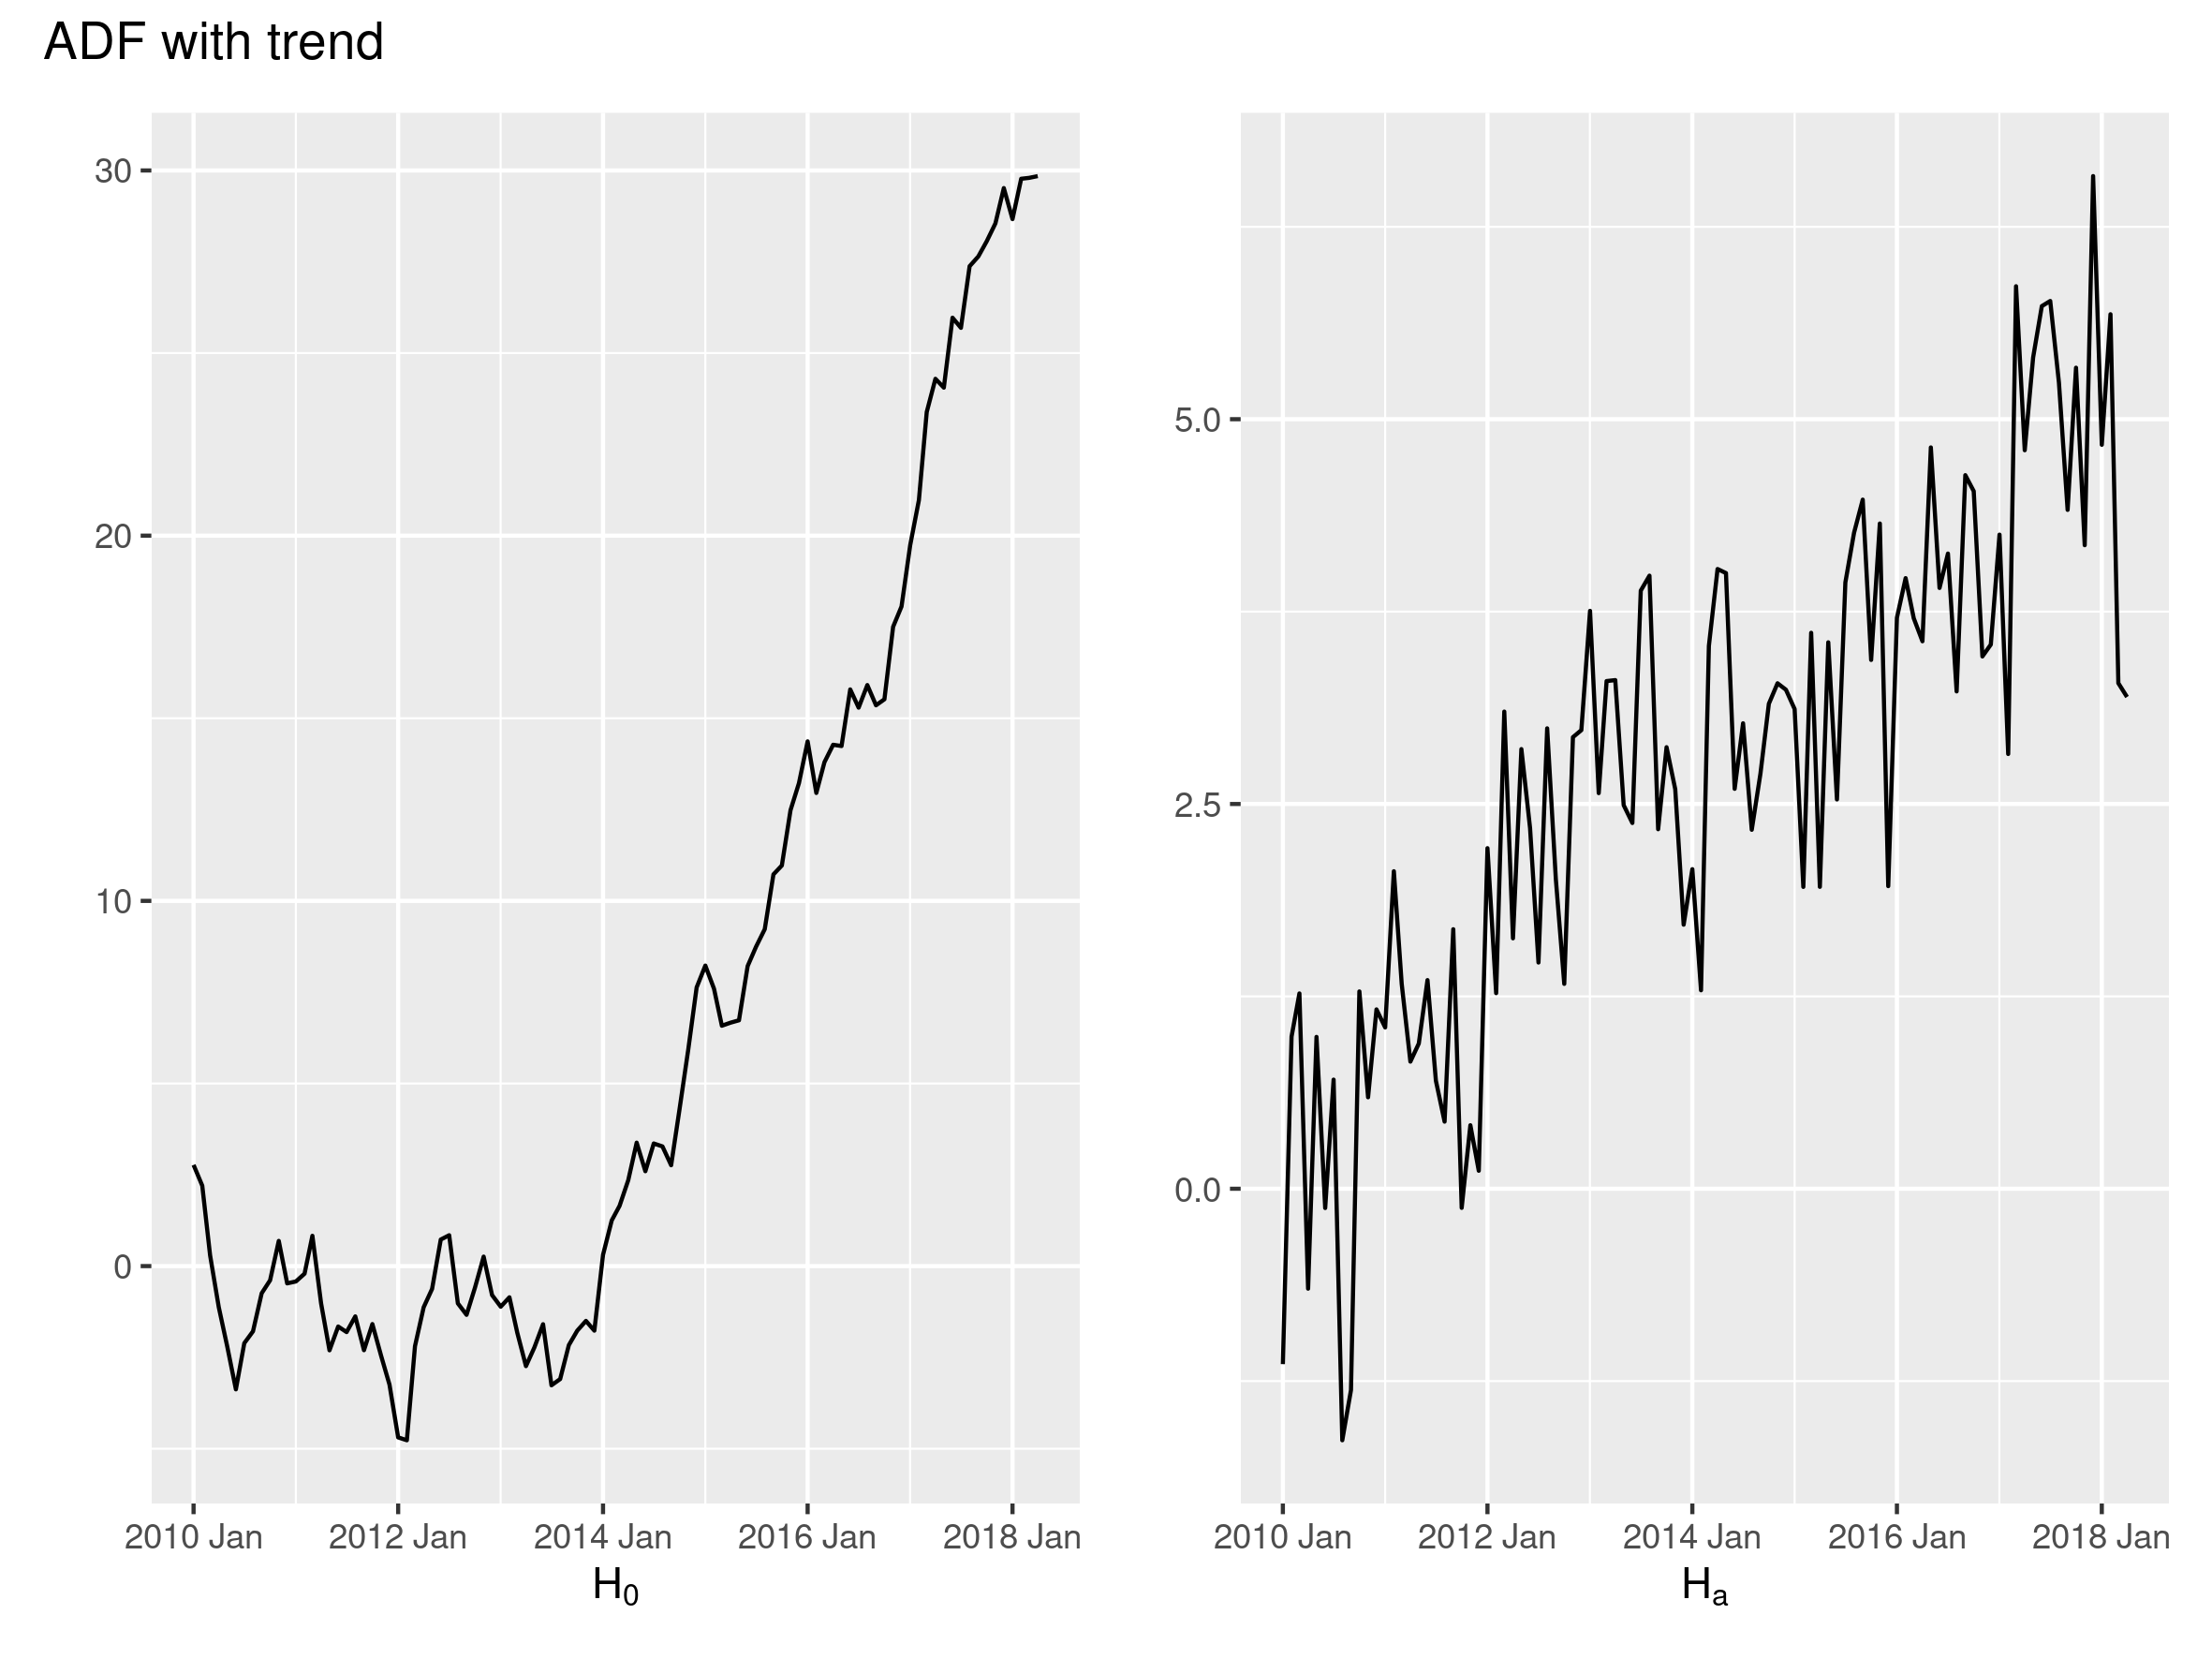
\includegraphics[width=\textwidth]{pictures/om_ts_06-060.png}
\end{frame}



\begin{frame}{$ADF$ test: Summary}
	
	\begin{itemize}[<+->]
		\item Applicable for making a decision about the transition to $\Delta y_t$
		\item Three variants of the ADF test with different assumptions		
	\end{itemize}
\end{frame}






\begin{frame} % frame name
	
	\videotitle{Unit root tests: KPSS test }
	
\end{frame}



\begin{frame}{KPSS test: Plan}
	\begin{itemize}[<+->]
		\item Long-term variance
		\item Prerequisites for the test
		\item Two variations of the test
	\end{itemize}
	
\end{frame}

\begin{frame}
	\frametitle{KPSS test}
	
	KPSS — \alert{Kwiatkowski–Phillips–Schmidt–Shin} test
	
	\pause
	Two variations of the test: with a constant, with a trend
	
\end{frame}


\begin{frame}
	\frametitle{Long-term variance}
	
	\begin{block}{Definition}
		For a stationary process $(y_t)$, the quantity $\lambda^2$ is called \alert{long-term variance} if
		\[
		\Var(\bar y) = \frac{\lambda^2}{T} + o(1/T)
		\]
		or
		\[
		\lim_{T \to \infty} T \Var(\bar y) = \lambda^2,
		\]
		where $\bar y = (y_1 + \ldots + y_T) / T$.
	\end{block}
	
	\pause
	
	\begin{block}{Motivation}
		For independent observations with the constant  variance
		\[
		\Var(\bar y) = \frac{\sigma^2}{T},\text{ where }\sigma^2 = \Var(y_i)
		\]
	\end{block}
	
\end{frame}


\begin{frame}
	\frametitle{KPSS with constant}
	\[
	y_t = c + rw_t + x_t,
	\]
	
	\pause
	
	\alert{$H_0$: $rw_t = 0$}
	
	$(x_t)$ is a stationary process with $\E(x_t) = 0$;
	
	\pause
	
	\alert{$H_a$: $rw_t = rw_{t-1} + u_t$}
	
	$rw_0 = 0$;
	
	$(x_t)$ is a stationary process with $\E(x_t) = 0$;
	
	$(u_t)$ is white noise independent of $(x_t)$
	
\end{frame}

\begin{frame}
	\frametitle{KPSS with constant: $H_0$ and $H_a$}
	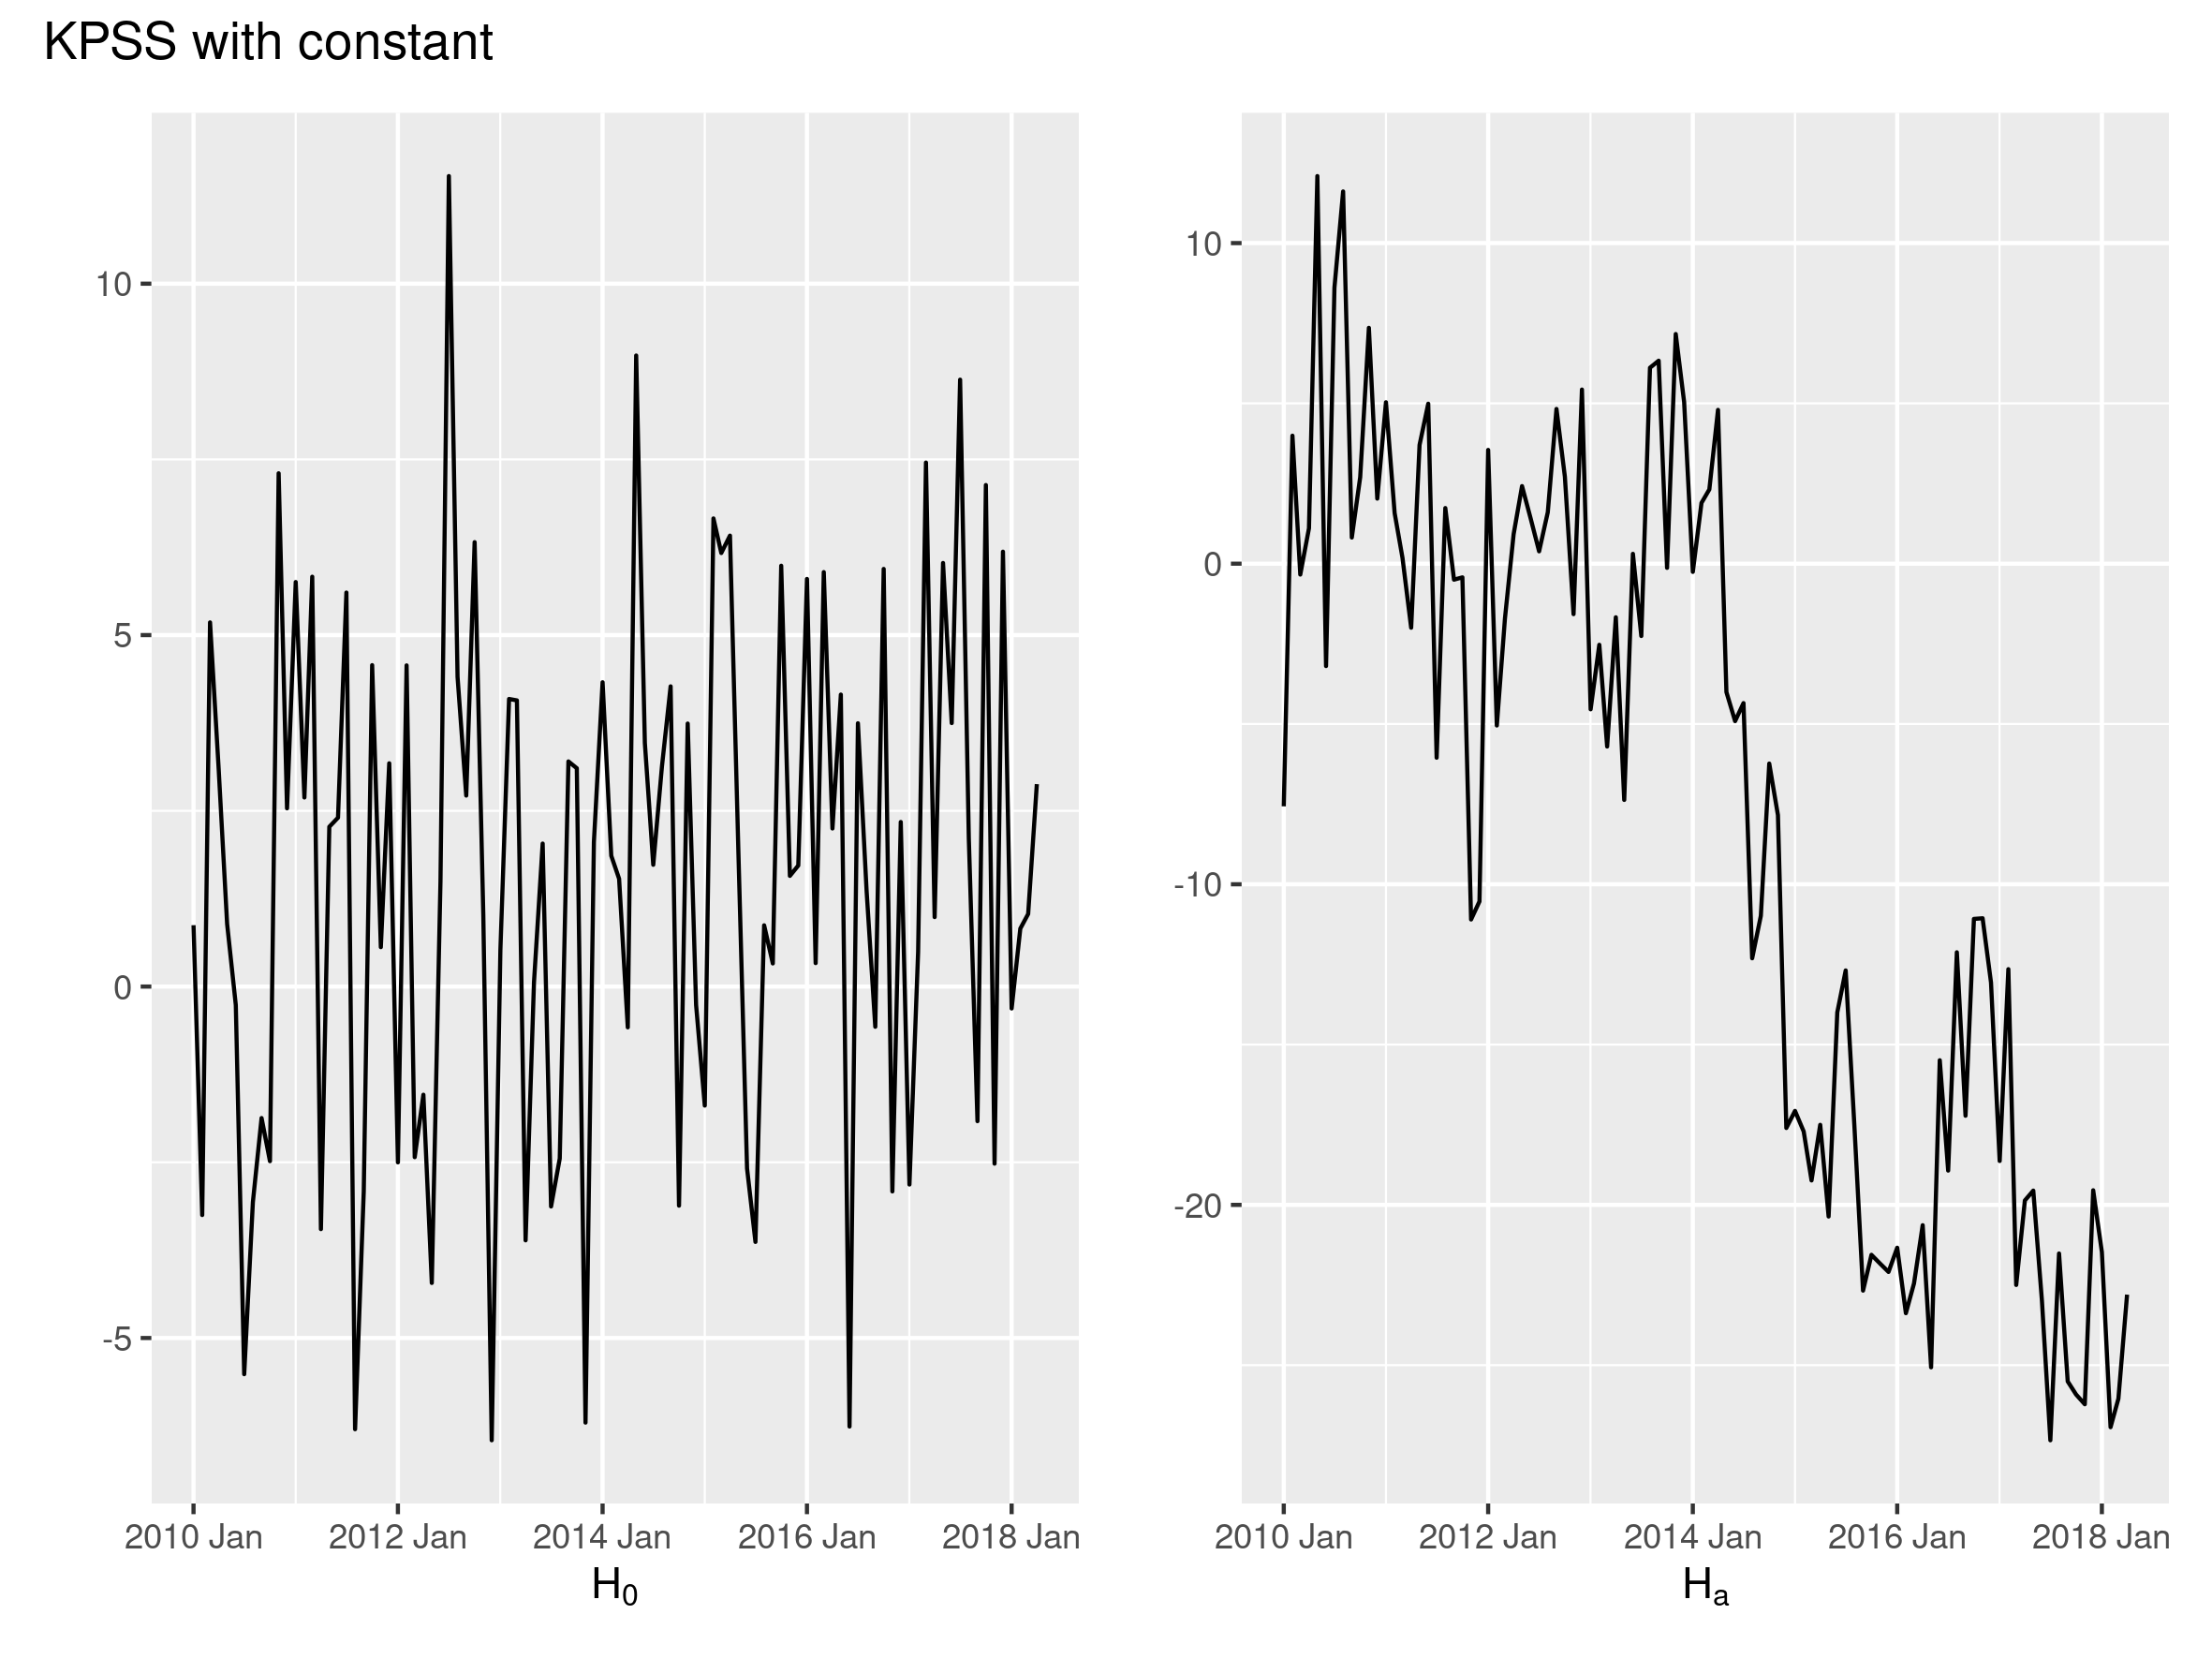
\includegraphics[width=\textwidth]{pictures/om_ts_06-077.png}
	
\end{frame}

\begin{frame}
	\frametitle{KPSS with constant: algorithm}
	
	Step 1. Evaluate regression on a \alert{constant }
	\[
	\widehat{y_t} = \hat c
	\]
	
	\pause
	Step 2. Calculate $KPSS$ statistics
	\[
	KPSS = \frac{\sum_{t=1}^T S_t^2}{T^2 \hat \lambda^2},
	\]
	where $S_t$ is the accumulated sum of residuals, $S_t = \hat u_1 + \ldots + \hat u_t$,
	
	and $\hat\lambda^2$ is a consistent estimator of the long-term variance.
	
	\pause
	Under true $H_0$, the distribution of the $KPSS$-statistic converges to a  \alert{special distribution} with $KPSS^c$!
	
	\pause
	Step 3. We conclude:
	
	If $KPSS > KPSS^c$ then $H_0$ is rejected
	
\end{frame}


\begin{frame}
	\frametitle{KPSS with trend}
	\[
	y_t = c + bt + rw_t + x_t,
	\]
	
	\pause
	
	\alert{$H_0$: $rw_t = 0$}
	
	$(x_t)$ is a stationary process with $\E(x_t) = 0$;
	
	\pause
	
	\alert{$H_a$: $rw_t = rw_{t-1} + u_t$}
	
	$rw_0 = 0$;
	
	$(x_t)$ is a stationary process with $\E(x_t) = 0$;
	
	$(u_t)$ is white noise independent of $(x_t)$
	
	\pause
	
	The first step of the algorithm will have a regression \alert{on a constant and a trend} and the statistic under null will have   another special distribution $KPSS^{ct}$
	
\end{frame}


\begin{frame}
	\frametitle{KPSS with trend: $H_0$ and $H_a$}
	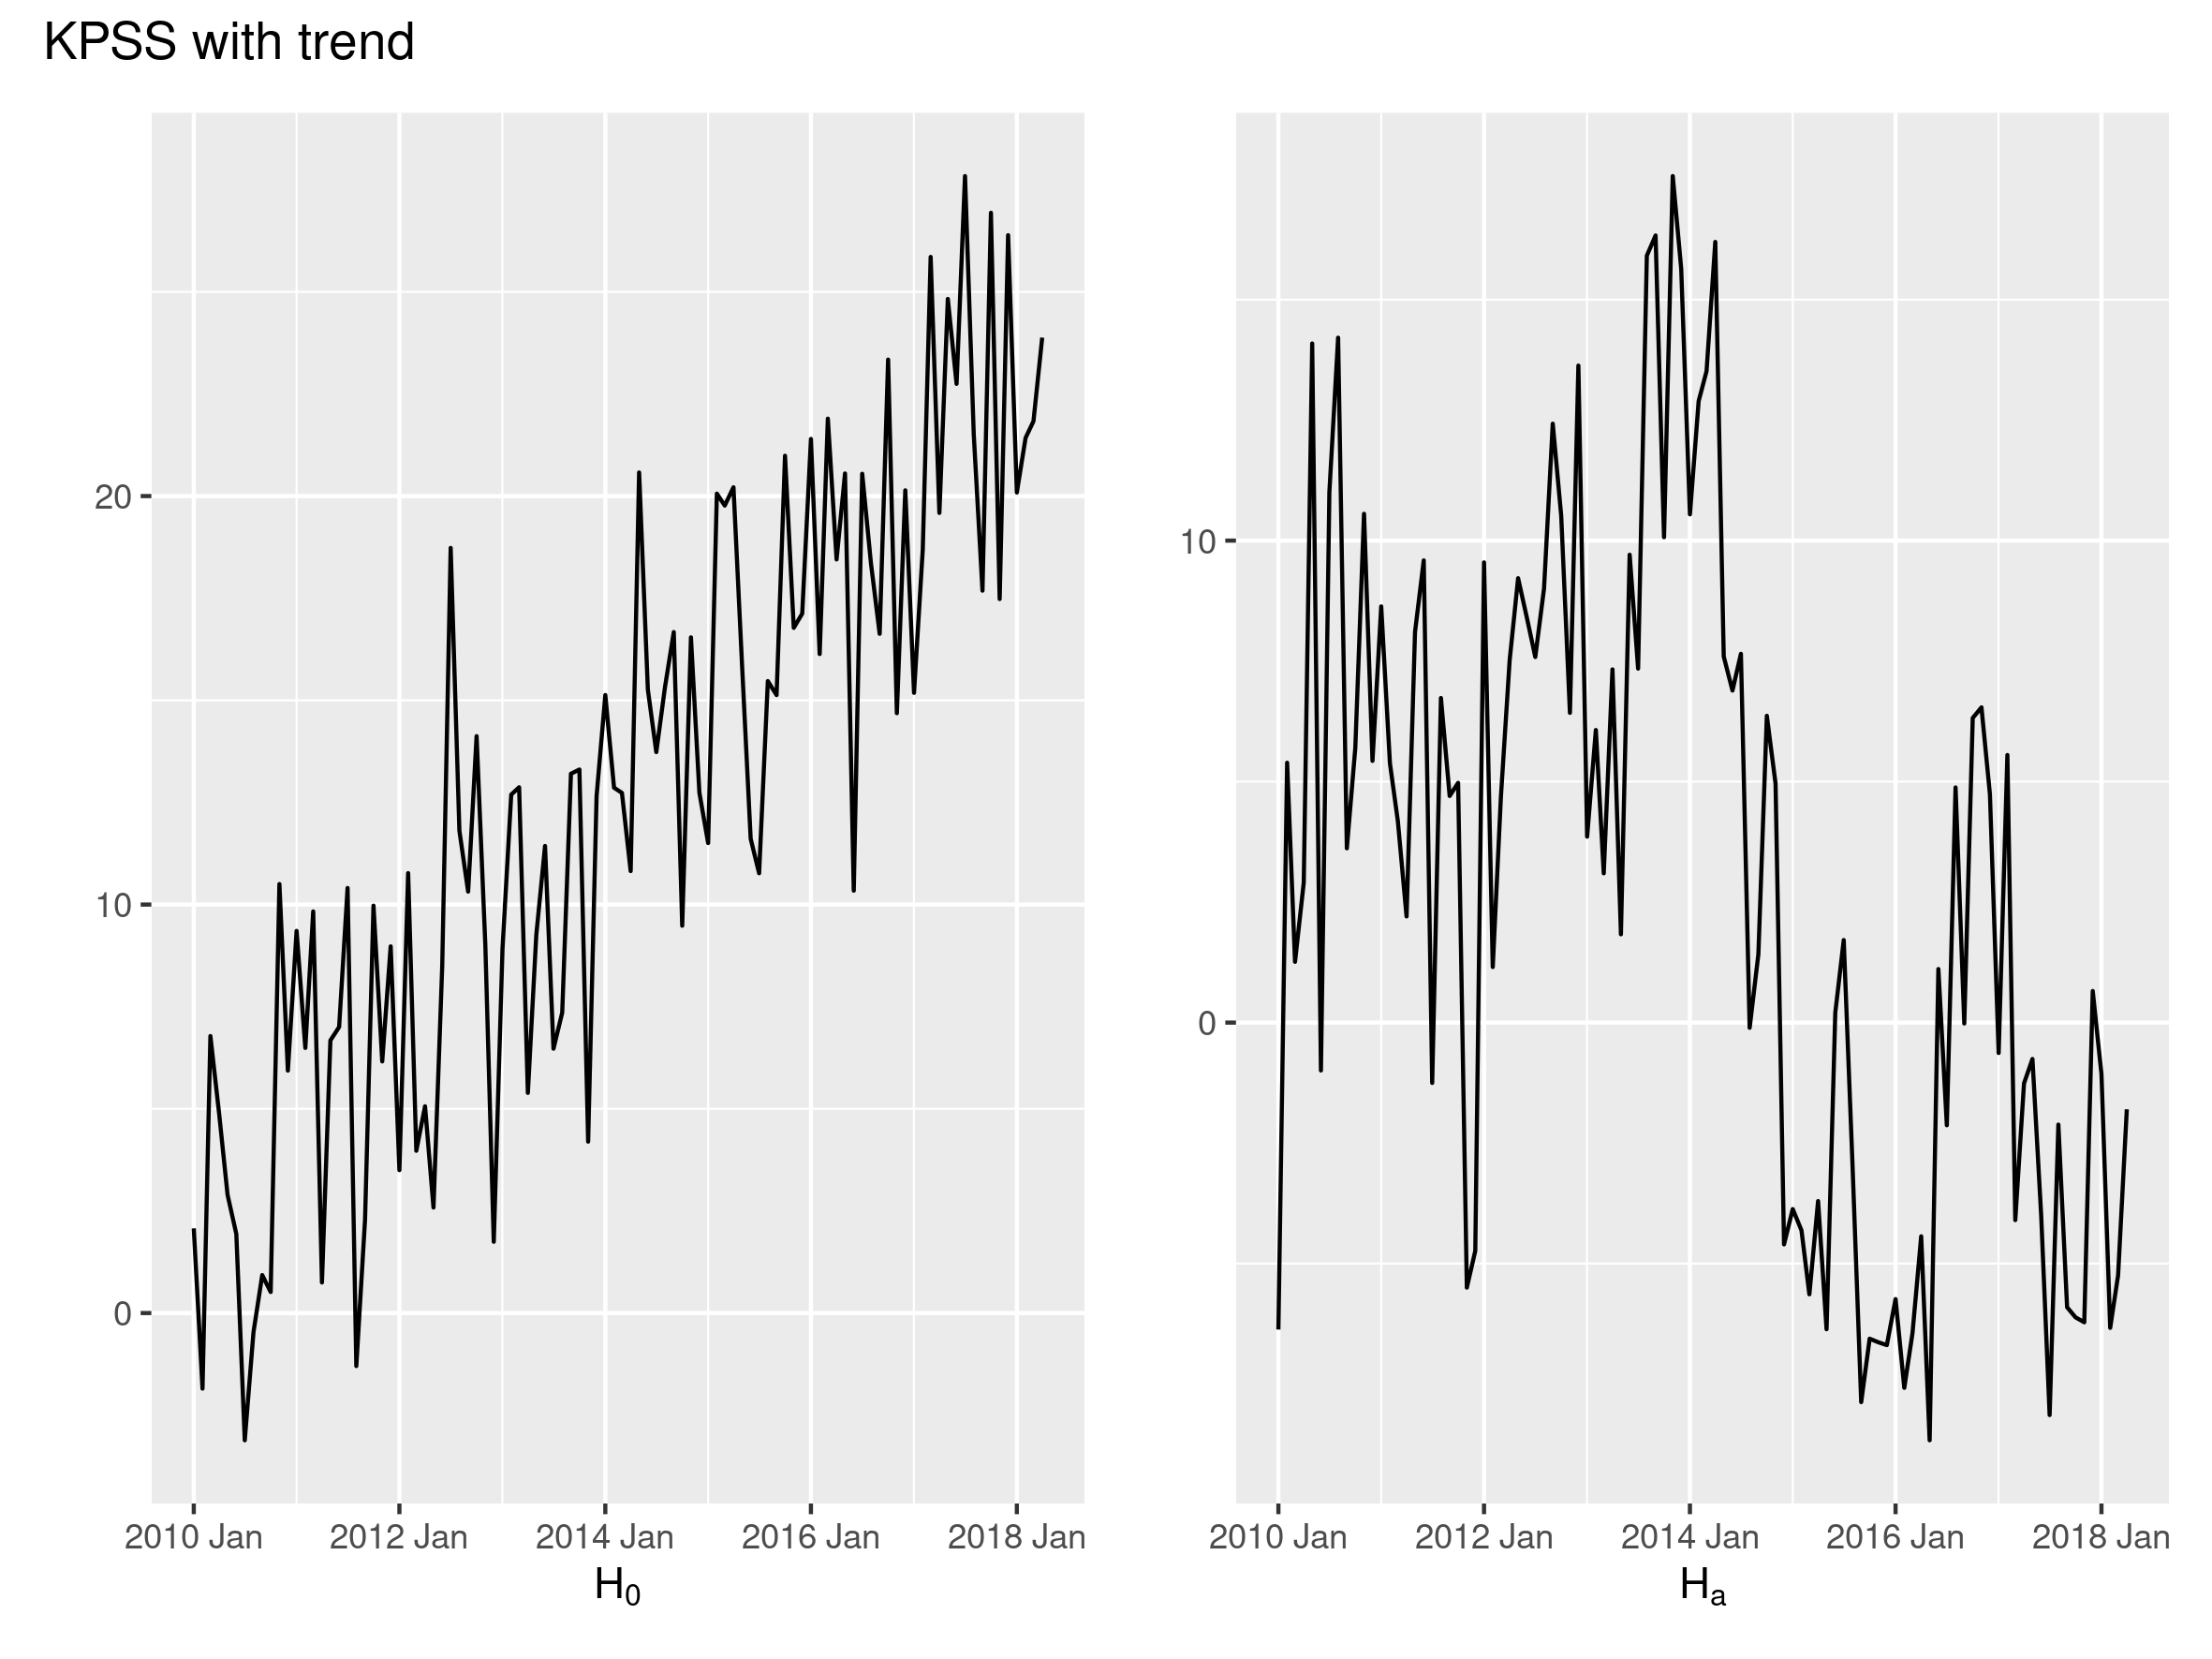
\includegraphics[width=\textwidth]{pictures/om_ts_06-086.png}
\end{frame}

% TODO: move A and B and highlight with color!
\begin{frame}
	\frametitle{Terminology}
	\[
	A. \quad y_t = a + bt + x_t
	\]
	
	$(y_t)$ — \alert{trend stationary} (stationary around the trend)
	
	$(x_t)$ — a stationary process with $\E(x_t) = 0$
	
	\pause Recipe: Estimate regression $a + bt$ with $ARMA$ errors for $(y_t)$.
	\pause
	\[
	B. \quad y_t = a + \sum_{i=1}^t x_i \text{ or } y_t = a + bt + \sum_{i=1}^t x_i
	\]
	
	$(x_t)$ — a stationary process with $\E(x_t) = 0$
	
	$(y_t)$ — \alert{difference stationary} (stationary in differences)
	
	\pause Recipe: evaluate $ARMA$ for $(\Delta y_t)$.
	
	\pause Both $(y_t)$ are non-stationary!
	
\end{frame}



\begin{frame}{KPSS test: Summary}
	
	\begin{itemize}[<+->]
		\item Applicable for making a decision about the transition to $\Delta y_t$
		\item Two versions of the KPSS test with different assumptions	
		
	\end{itemize}
\end{frame}







\end{document}
